\documentclass{beamer}

\mode<presentation> {
\usetheme[secheader]{Madrid}
\usecolortheme{seahorse}
\useinnertheme{circles}
}

\usepackage{graphicx} % Allows including images
\usepackage{booktabs} % Allows the use of \toprule, \midrule and \bottomrule in tables
\usepackage{tikz}
\usepackage{caption}
\usepackage{hyperref}

\setbeamerfont{section in sidebar}{size=\fontsize{5}{6}\selectfont}
\setbeamerfont{subsection in sidebar}{size=\fontsize{3}{5}\selectfont}
\setbeamerfont{subsubsection in sidebar}{size=\fontsize{2}{4}\selectfont}

\usepackage{tcolorbox}


%----------------------------------------------------------------------------------------
%	TITLE PAGE
%----------------------------------------------------------------------------------------

\makeatletter
%\patchcmd{\beamer@sectionintoc}{\vskip1.5em}{\vskip0.5em}{}{}
%\patchcmd{\beamer@subsectionintoc}{\vskip1.5em}{\vskip0.5em}{}{}
\makeatother



\title[HCI x AI]{HCI x AI} % The short title appears at the bottom of every slide, the full title is only on the title page

\author{Chaklam Silpasuwanchai, Pranisaa Charnparttaravanit} % Your name
\institute[AIT] % Your institution as it will appear on the bottom of every slide, may be shorthand to save space
{
Asian Institute of Technology \\ % Your institution for the title page
\medskip
\textit{chaklam@ait.asia} % Your email address
}
\date{} % Date, can be changed to a custom date

\AtBeginSection[]
{
\begin{frame}<beamer> 
\tableofcontents[currentsection]  % show TOC and highlight current section
\end{frame}
}

\begin{document}

\begin{frame}
\titlepage % Print the title page as the first slide
\end{frame}

\begin{frame}
\frametitle{Overview} % Table of contents slide, comment this block out to remove it
\footnotesize
\tableofcontents
 % Throughout your presentation, if you choose to use \section{} and \subsection{} commands, these will automatically be printed on this slide as an overview of your presentation
\end{frame}

%----------------------------------------------------------------------------------------
%	PRESENTATION SLIDES
%----------------------------------------------------------------------------------------

\begin{frame}
\frametitle{Sources} 
\begin{itemize}
	\item CHI Conference Proceedings
    \item ACL, EMNLP Conference Proceedings
    \item Some from preprint like arxiv
\end{itemize}
\end{frame}

\begin{frame}
\frametitle{My intention} 
\begin{itemize}
	\item Focus on \textbf{how people do research}, particularly on \textbf{experimental} studies - how they choose IV, DV, etc.
    \item As you will see, most important is \textbf{creativity} and \textbf{a very rigorous experimental study}.
    \item All have very deep \textbf{discussion}, showing how smart they are.
    \item One good figure, and good video.
    \item If you like more \textit{engineering},  we will talk more in next year class \textbf{NLP} and read more from the \textbf{ACL} conference!
\end{itemize}
\end{frame}

%------------------------------------------------
\section{Human AI Interaction} % Sections can be created in order to organize your presentation into discrete blocks, all sections and subsections are automatically printed in the table of contents as an overview of the talk

\begin{frame}
    \frametitle{Human-AI Interaction: What is it?}
    \footnotesize
    
    \begin{center}
        \textbf{Basically, a field where \textcolor{orange}{Humans} and \textcolor{green}{AIs} \textcolor{blue}{interact}.}
    \end{center}
    
    \vspace{0.5cm}
    
    \begin{itemize}
        \item \textbf{\textcolor{orange}{Humans}}: AI researchers, model developers, domain experts, end users.
        \item \textbf{\textcolor{green}{AIs}}: dialog system, translator, recommender system, autonomous driving system.
        \item \textbf{\textcolor{blue}{Interact}}:
        \begin{itemize}
            \item Humans collaborate with AI 
            \item Humans get assistance from AI-infused applications
        \end{itemize}
    \end{itemize}
\end{frame}

\begin{frame}
    \frametitle{Human-AI Collaboration}
    \footnotesize
    
    \begin{center}
        \begin{minipage}{0.45\textwidth}
            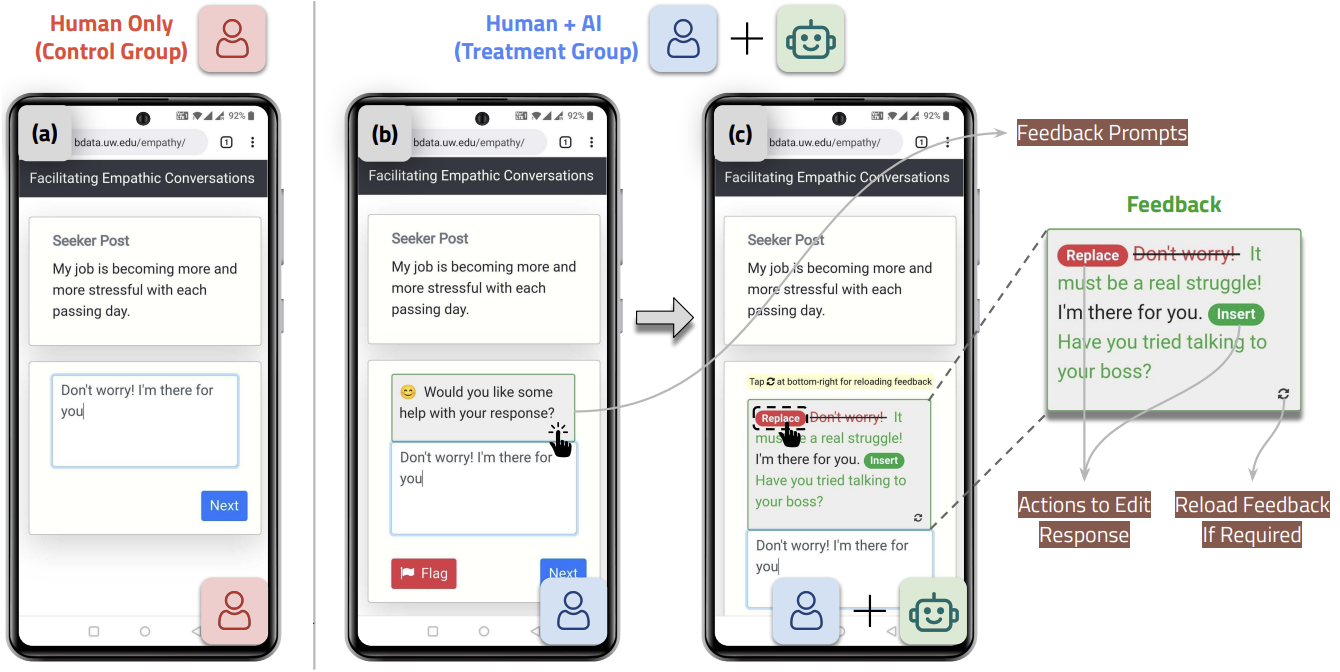
\includegraphics[width=\linewidth]{helping.png}
            \textit{Empathic
Conversations in Text-based Peer-to-Peer Mental
Health Support}
        \end{minipage}\hfill
        \begin{minipage}{0.45\textwidth}
            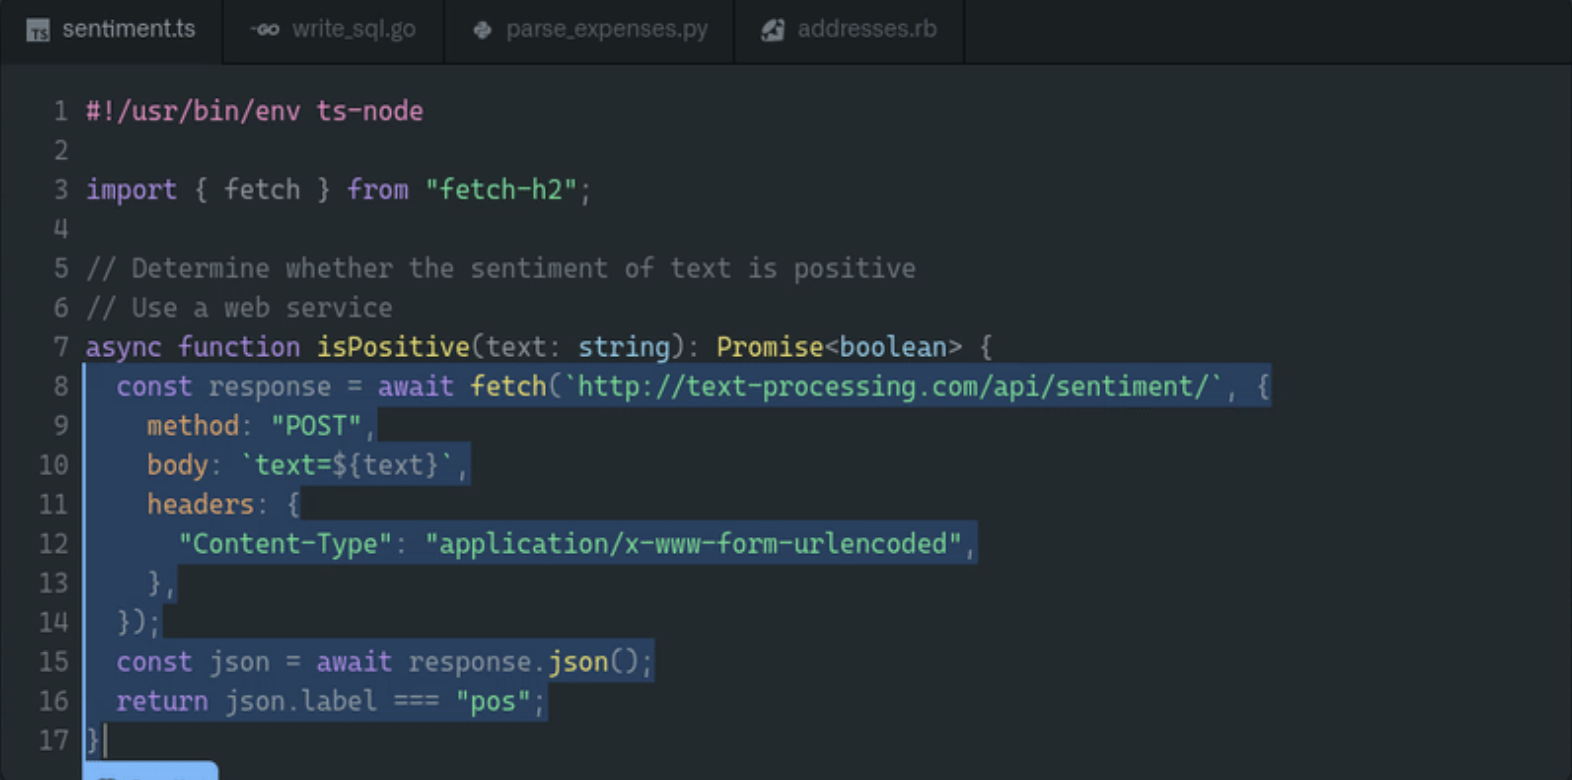
\includegraphics[width=\linewidth]{copilot.png}
            \textit{Co-pilot}
        \end{minipage}\hfill
        % \begin{minipage}{0.3\textwidth}
        %     \includegraphics[width=\linewidth]{image3.png}
        % \end{minipage}
    \end{center}
    
\end{frame}


\begin{frame}
    \frametitle{Human-AI Collaboration}
    \footnotesize
    
    \begin{itemize}
        \item How do we shape these collaborations in ways that are meaningful, productive, and intuitive?
        % \vspace{1.0cm}
        % \item What are key aspects to create meaningful collaboration?
    \end{itemize}
\end{frame}

% \begin{frame}
%     \frametitle{Human-AI Collaboration: Example applications}
%     \footnotesize
    
%     \begin{itemize}
%         \item What are Human-AI Collaboration applications in your daily life?
%         \vspace{1.0cm}
%         \item What are key aspects to consider?
%     \end{itemize}
% \end{frame}

\begin{frame}
    \frametitle{Human-AI Collaboration: key aspects}
    \footnotesize

%     \begin{center}
%         The \textcolor{gray}{cooperative} and \textcolor{gray}{coordinated} interaction between humans \textcolor{blue}{(mostly non-AI
% experts)} and AI to solve \textit{complex problems or achieve certain goals.}
%     \end{center}

    \vspace{0.5cm}

    
    \begin{itemize}
        \item \textbf{Complementary performance}: Leverage the strengths of both AI and humans, to achieve better outcomes than either could accomplish alone.
        
        \item \textbf{Alignment}: AI should behave in ways that humans expect their ``teammate'' to behave.
        
        \item \textbf{Cooperative interaction}: The interaction between human and AI should work in a way that's both intuitive for the human, and compatible to model characteristics.
        
        \item \textbf{Reasonable task allocation}: Assign tasks that the model can perform.
        
        \item \textbf{Appropriate trust}: Humans should follow AIs when they are correct, but identify and correct their mistakes otherwise.
    \end{itemize}
\end{frame}

% \begin{frame}
%     \frametitle{Work with LLM: Account for model characteristics}
%     \footnotesize
    
%     \vspace{1cm} % adds the vertical space like in the screenshot
    
%     \begin{itemize}
%         \item Language models are not deterministic.
%         \item Language models lack reasoning capabilities.
%         \item Language models sometimes cannot understand instructions.
%     \end{itemize}
% \end{frame}


% \begin{frame}
%     \frametitle{Social Skill Training with Large Language Models (Yang, ACL 2025)\footnote{\tiny Yang, D. (2025). \textit{Social Skill Training with Large Language Models} ACL 2025.}}
%     \footnotesize
%     \centering
%     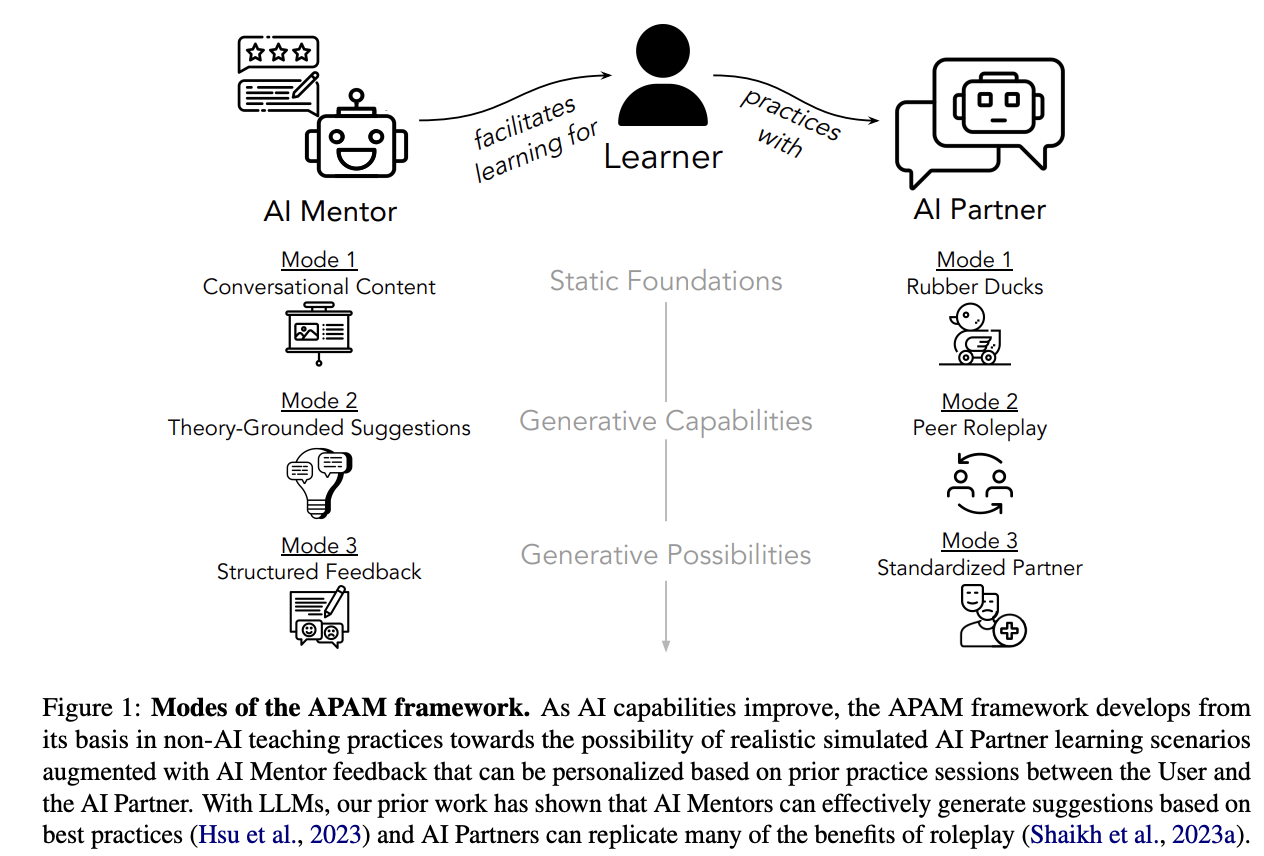
\includegraphics[width=0.75\linewidth]{sociallearning.png}
    % \begin{columns}
    %     % Left column
    %     \begin{column}{0.55\textwidth}
    %         \begin{itemize}
    %             \item \textbf{Motivation}: XXXX Examine whether AI-edited images/videos can distort memory or create false memories.
    %             \item \textbf{Task}: XXXX Participants viewed media (images/videos) and later recalled specific details.
    %             \item \textbf{IVs}: XXXX Type of media (original vs AI-edited), subtlety of edits (obvious vs subtle).  
    %             \item \textbf{DV}: XXXX Number of false memories, accuracy of recalled details.  
    %             \item \textbf{Participants}: XXXX 120 participants.
    %         \end{itemize}
    %     \end{column}
        
    %     % Right column
    %     \begin{column}{0.45\textwidth}
    %         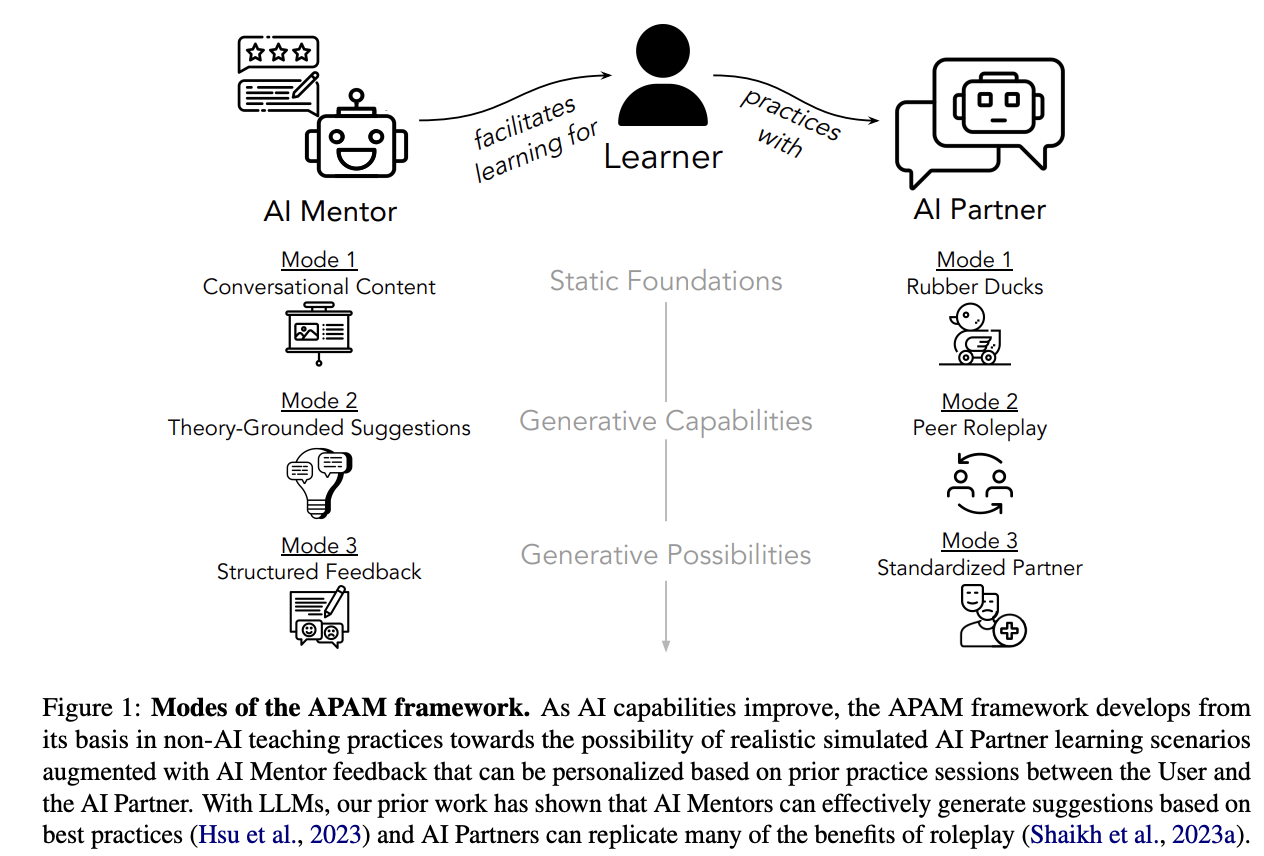
\includegraphics[width=\linewidth]{sociallearning.png}
    %         \item \url{xxx}
    %         \begin{itemize}
    %             \scriptsize
    %             \item XXXX AI-edited media caused more false memories than original content.  
    %             \item XXXX Subtle edits were sometimes more deceptive than obvious ones.  
    %             \item XXXX Implication: Critical media literacy is important when interacting with AI-generated content.
    %         \end{itemize}
    %     \end{column}
    % \end{columns}
% \end{frame}

\begin{frame}
    \frametitle{Rehearsal (Shaikh, SU, CHI 2024)\footnote{\tiny Shaikh, O. (2024). \textit{Rehearsal: Simulating Conflict to Teach Conflict Resolution} CHI 2024.}}
    \footnotesize
    \begin{columns}
        % Left column
        \begin{column}{0.55\textwidth}
        \vspace{-0.5em}
            \begin{itemize}
                \item \textbf{Goal}: To provide scalable, cost-effective conflict resolution training, addressing the scarcity of effective expert-led training 
                \item \textbf{System}: Interactive system that uses LLM grounded in conflict theory (Interest-Right-Power framework) to simulate realistic conflict.
                \begin{itemize}
                \item \textbf{simulates} realistic conflict
                \item allows people to \textbf{explore counterfactuals}
                \item \textbf{teaches} people conflict resoluation through deliberate practice
                \end{itemize}
                \item \url{https://www.youtube.com/watch?v=tLzKwHp_aeU}
            \end{itemize}
        \end{column}
        
        % Right column
        \begin{column}{0.45\textwidth}
            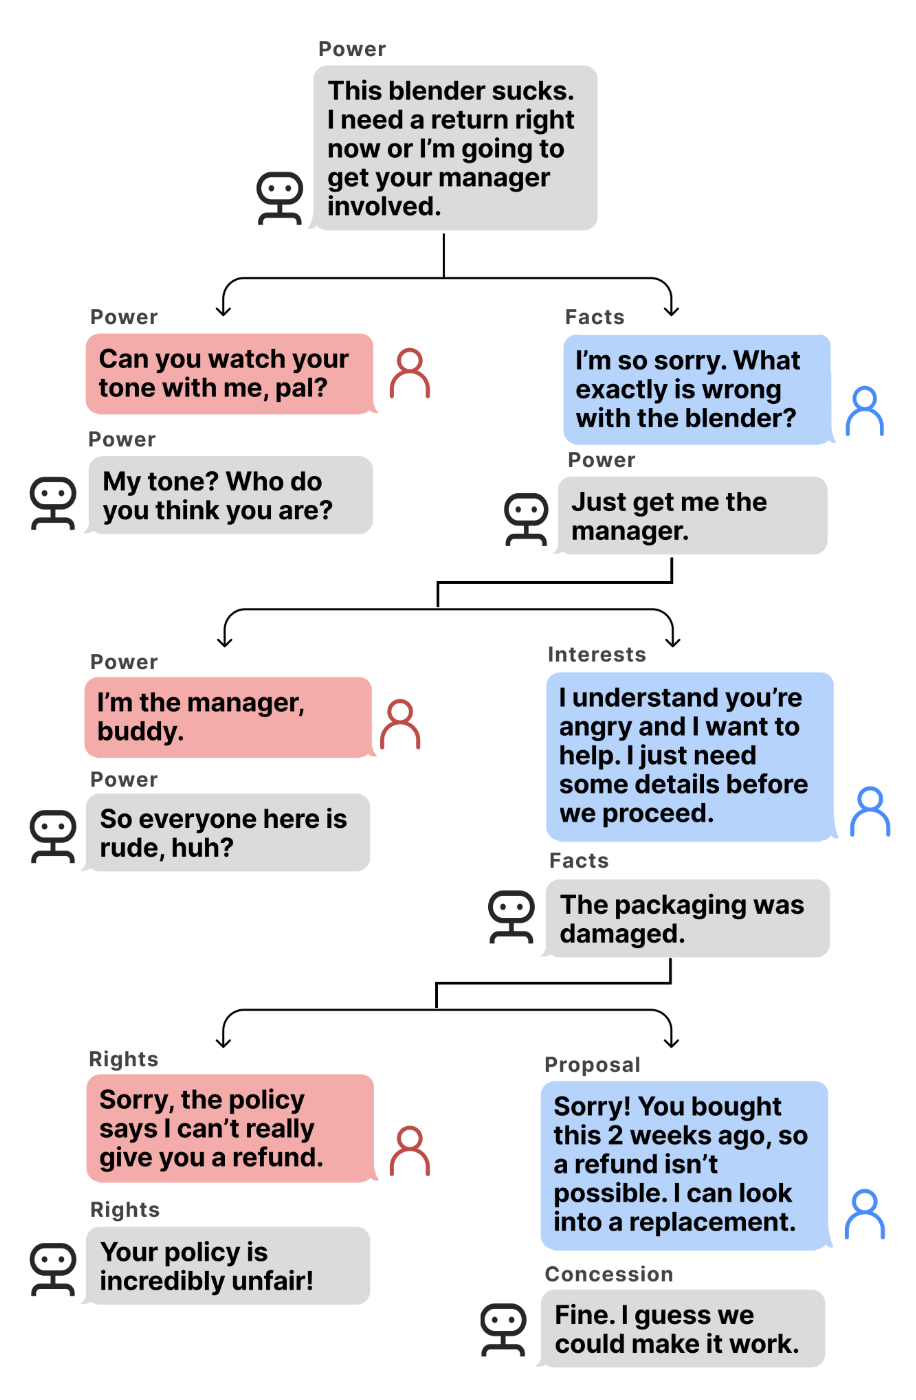
\includegraphics[width=0.85\linewidth]{rehearsal2.png}
        \end{column}
    \end{columns}
\end{frame}

% \begin{frame}
%     \frametitle{Rehearsal Conti ... (Shaikh, SU, CHI 2024)\footnote{\tiny Shaikh, O. (2024). \textit{Rehearsal: Simulating Conflict to Teach Conflict Resolution} CHI 2024.}}
%     \footnotesize

%     Simulate \textcolor{red}{Angry} People Interaction
%     \par\vspace{0.5cm} % <-- gap between text and image

%     % keep centering local to the image
%     {\centering
%     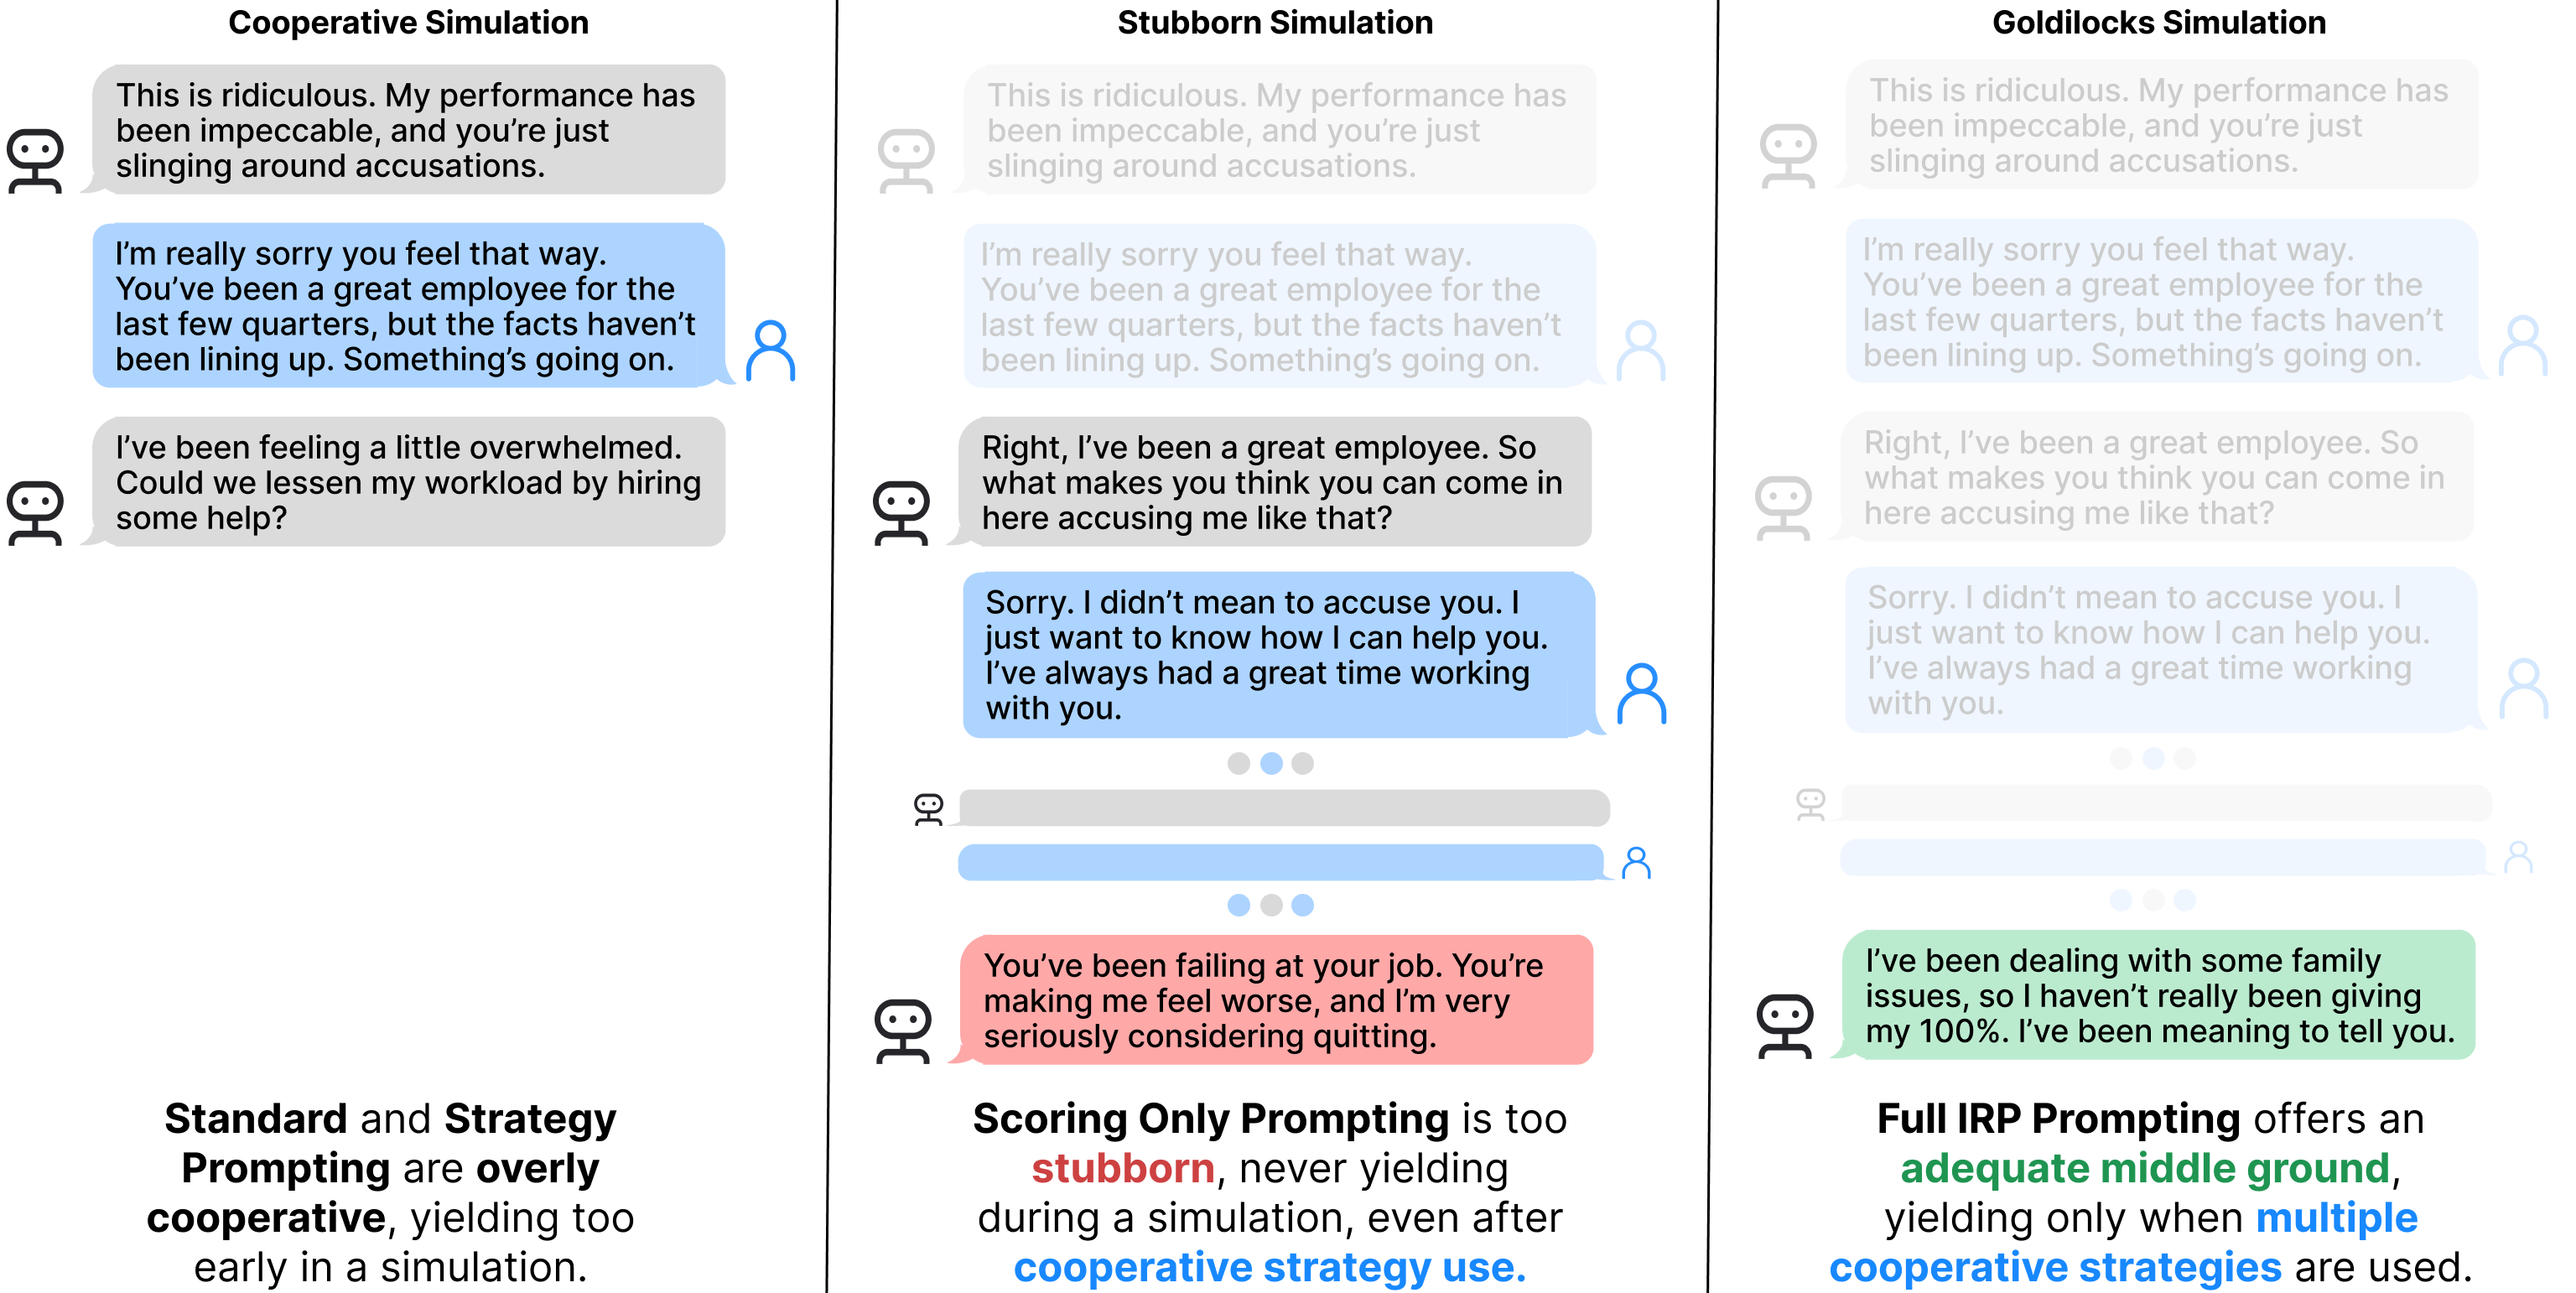
\includegraphics[width=0.85\linewidth]{rehearsal3.png}\par}
    
% \end{frame}

% \begin{frame}
%     \frametitle{Rehearsal Conti ... (Shaikh, SU, CHI 2024)\footnote{\tiny Shaikh, O. (2024). \textit{Rehearsal: Simulating Conflict to Teach Conflict Resolution} CHI 2024.}}
%     \footnotesize
%     Response Generating \& Scoring
%     \centering
%     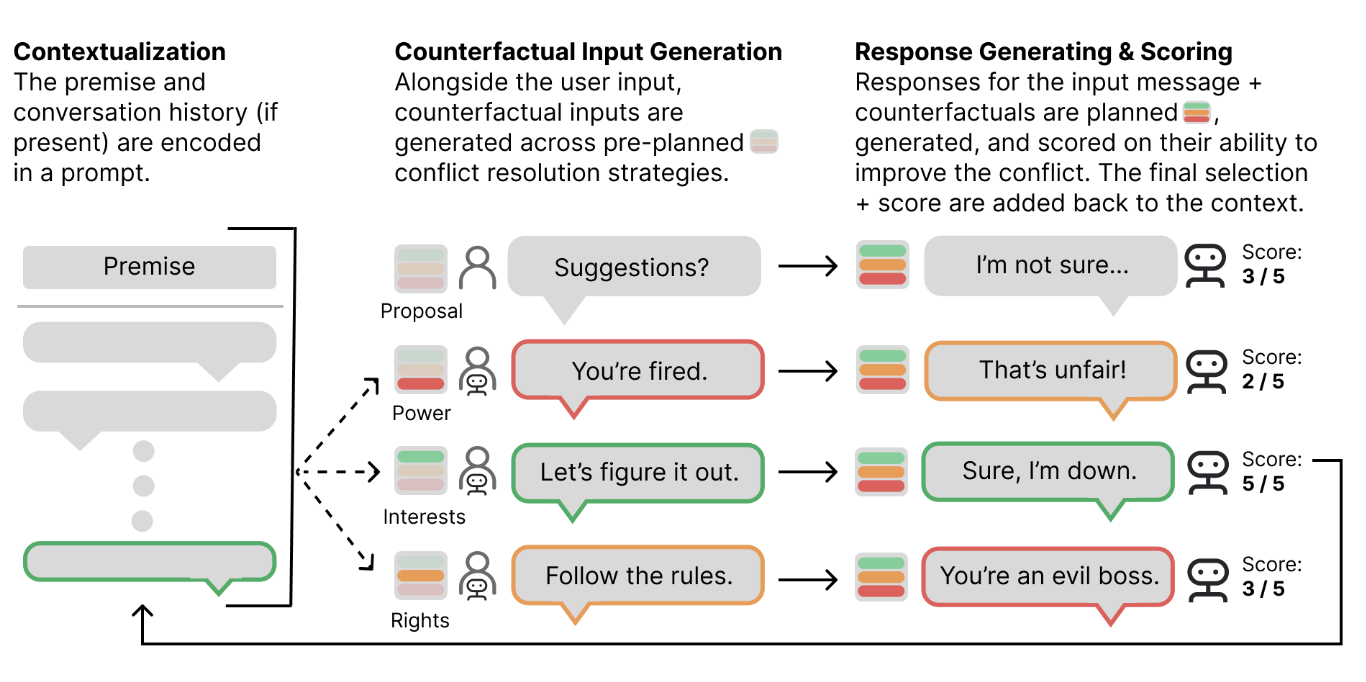
\includegraphics[width=0.85\linewidth]{rehearsal4.png}
% \end{frame}

\begin{frame}
    \frametitle{Rehearsal Conti ... (Shaikh, SU, CHI 2024)\footnote{\tiny Shaikh, O. (2024). \textit{Rehearsal: Simulating Conflict to Teach Conflict Resolution} CHI 2024.}}
    \footnotesize
    % 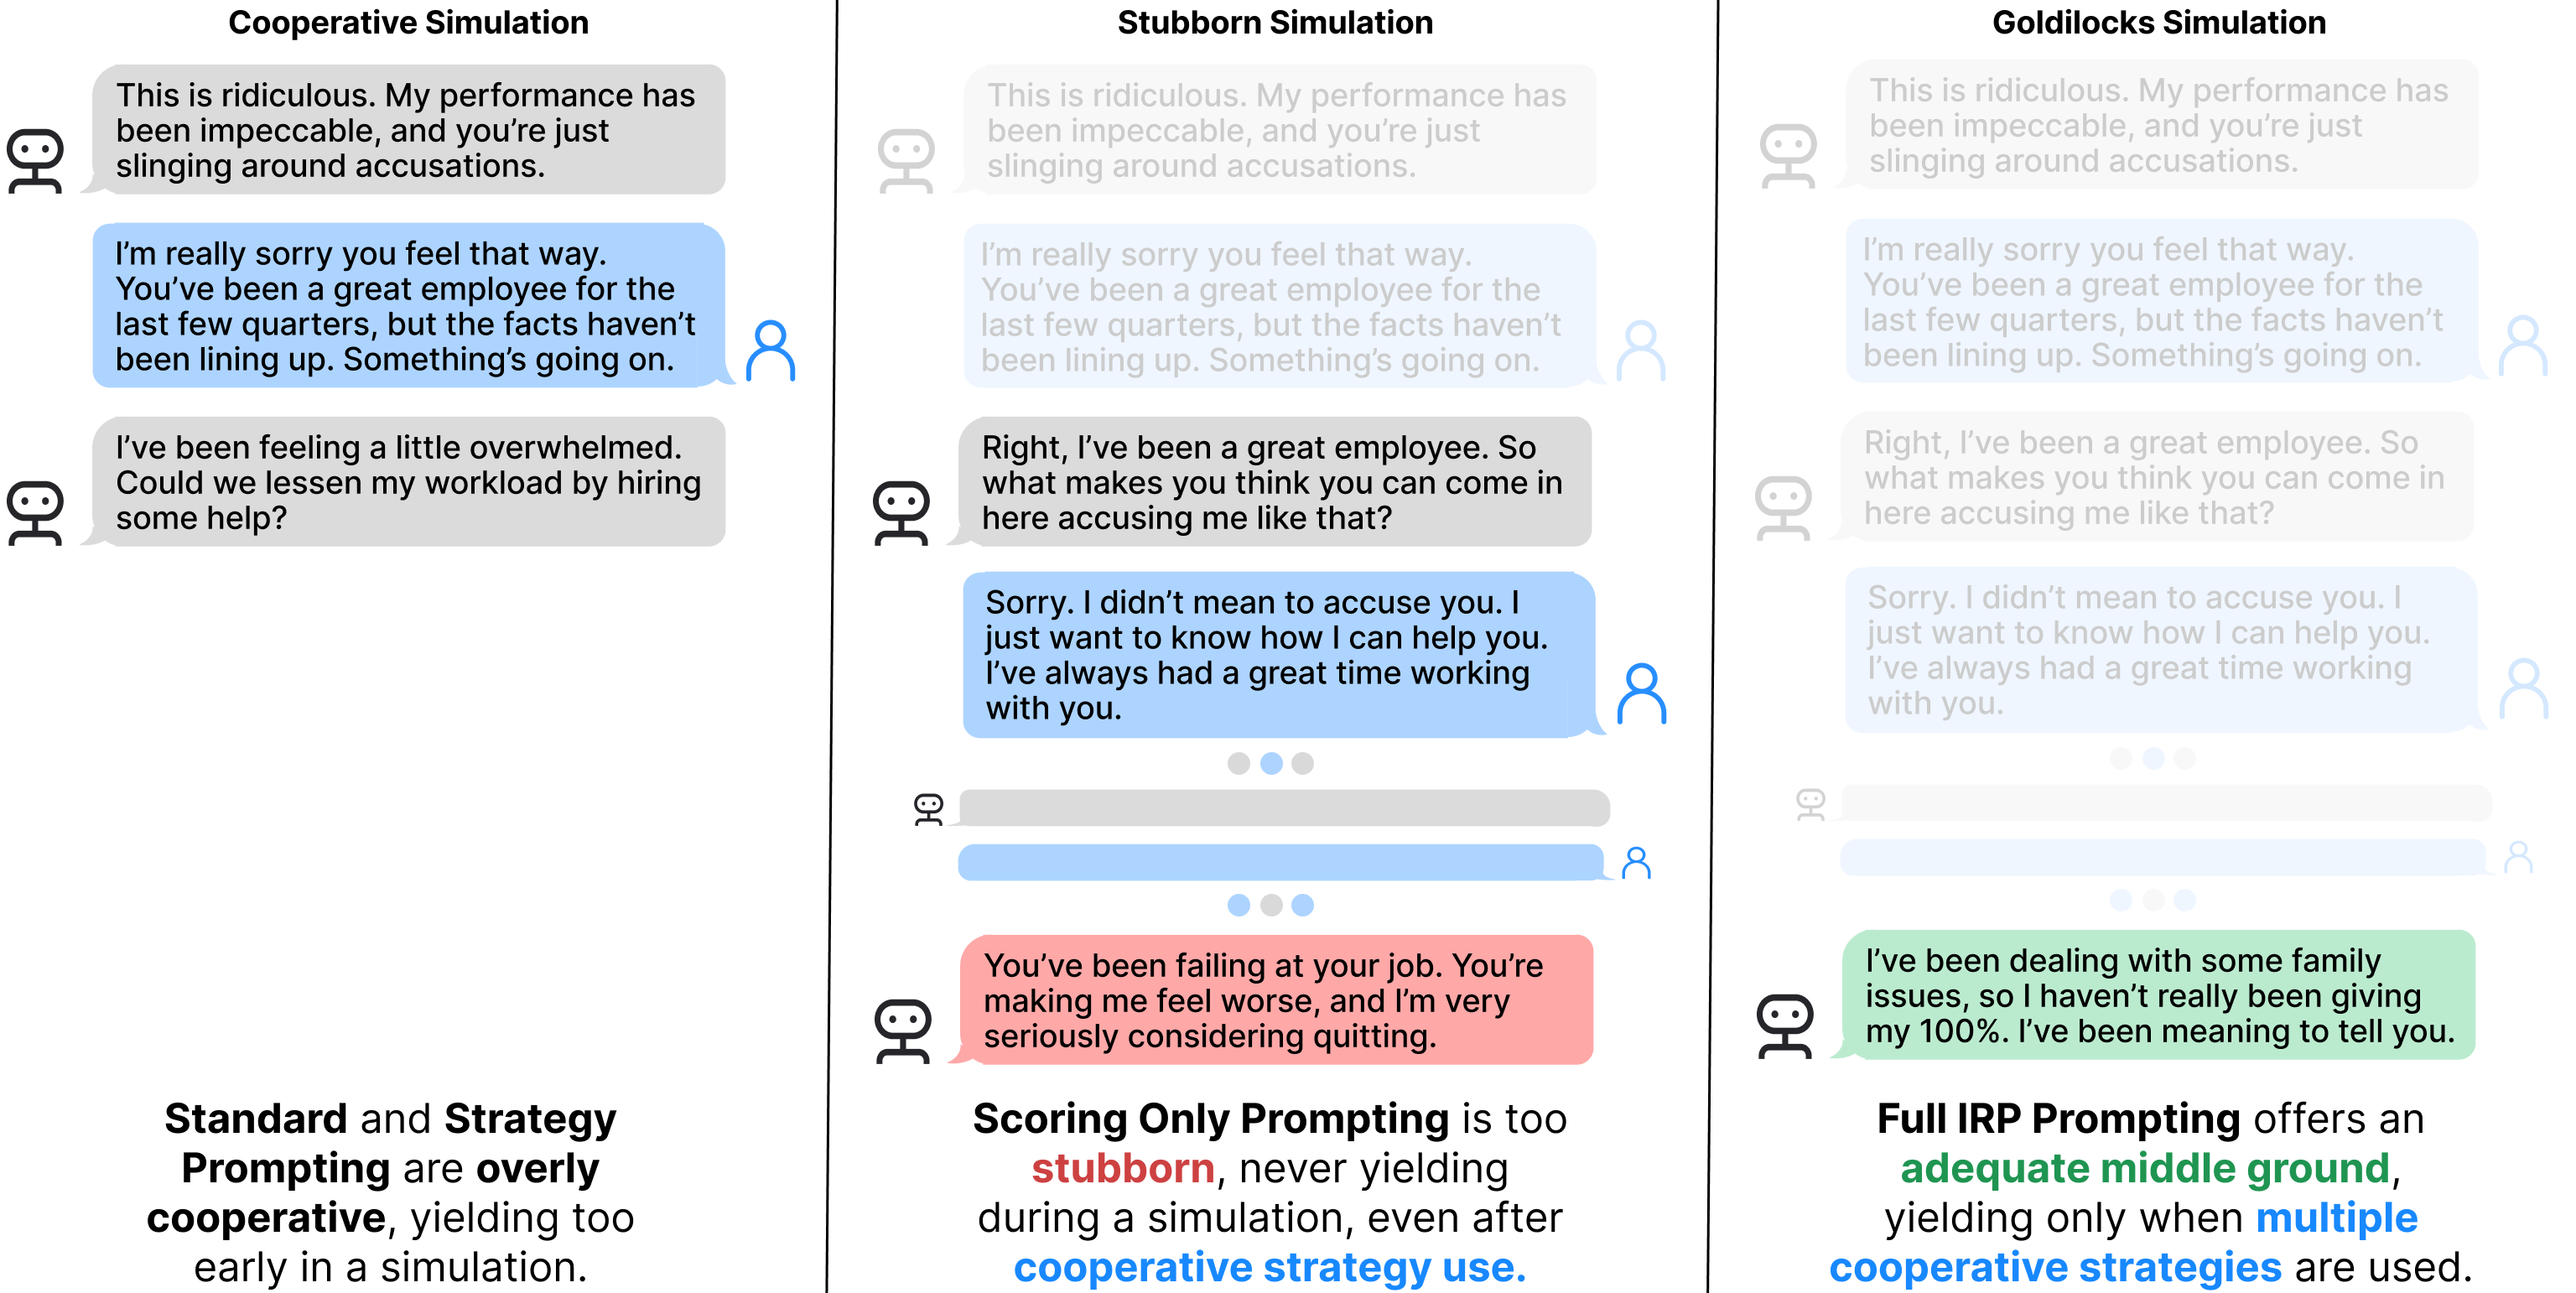
\includegraphics[width=0.85\linewidth]{rehearsal3.png}
    \begin{columns}
        % Left column
        \begin{column}{0.55\textwidth}
            \begin{itemize}
                \item \textbf{IVs}: Type of learning medium (4-min lecture video on IRP framework vs Rehearsal)
                \item \textbf{DV}: IRP strategy classification accuracy, Frequency of using Interest strategies (cooperative) and Right-Power strategies (competitive) , Conflict self-efficacy using pre-post study surveys
                \item \textbf{Participants}: 40 participants.
                \item \textbf{Key Findings}:
                \begin{itemize}
                \scriptsize
                \item Not significant on improving IRP strategy classification 
                \item Doubled cooperative strategies used and reduce the use of competitive strategies by 67 \%  
                \item Hard to implement in real situation
                \end{itemize}
            \end{itemize}
        \end{column}
        
        % Right column
        \begin{column}{0.45\textwidth}
            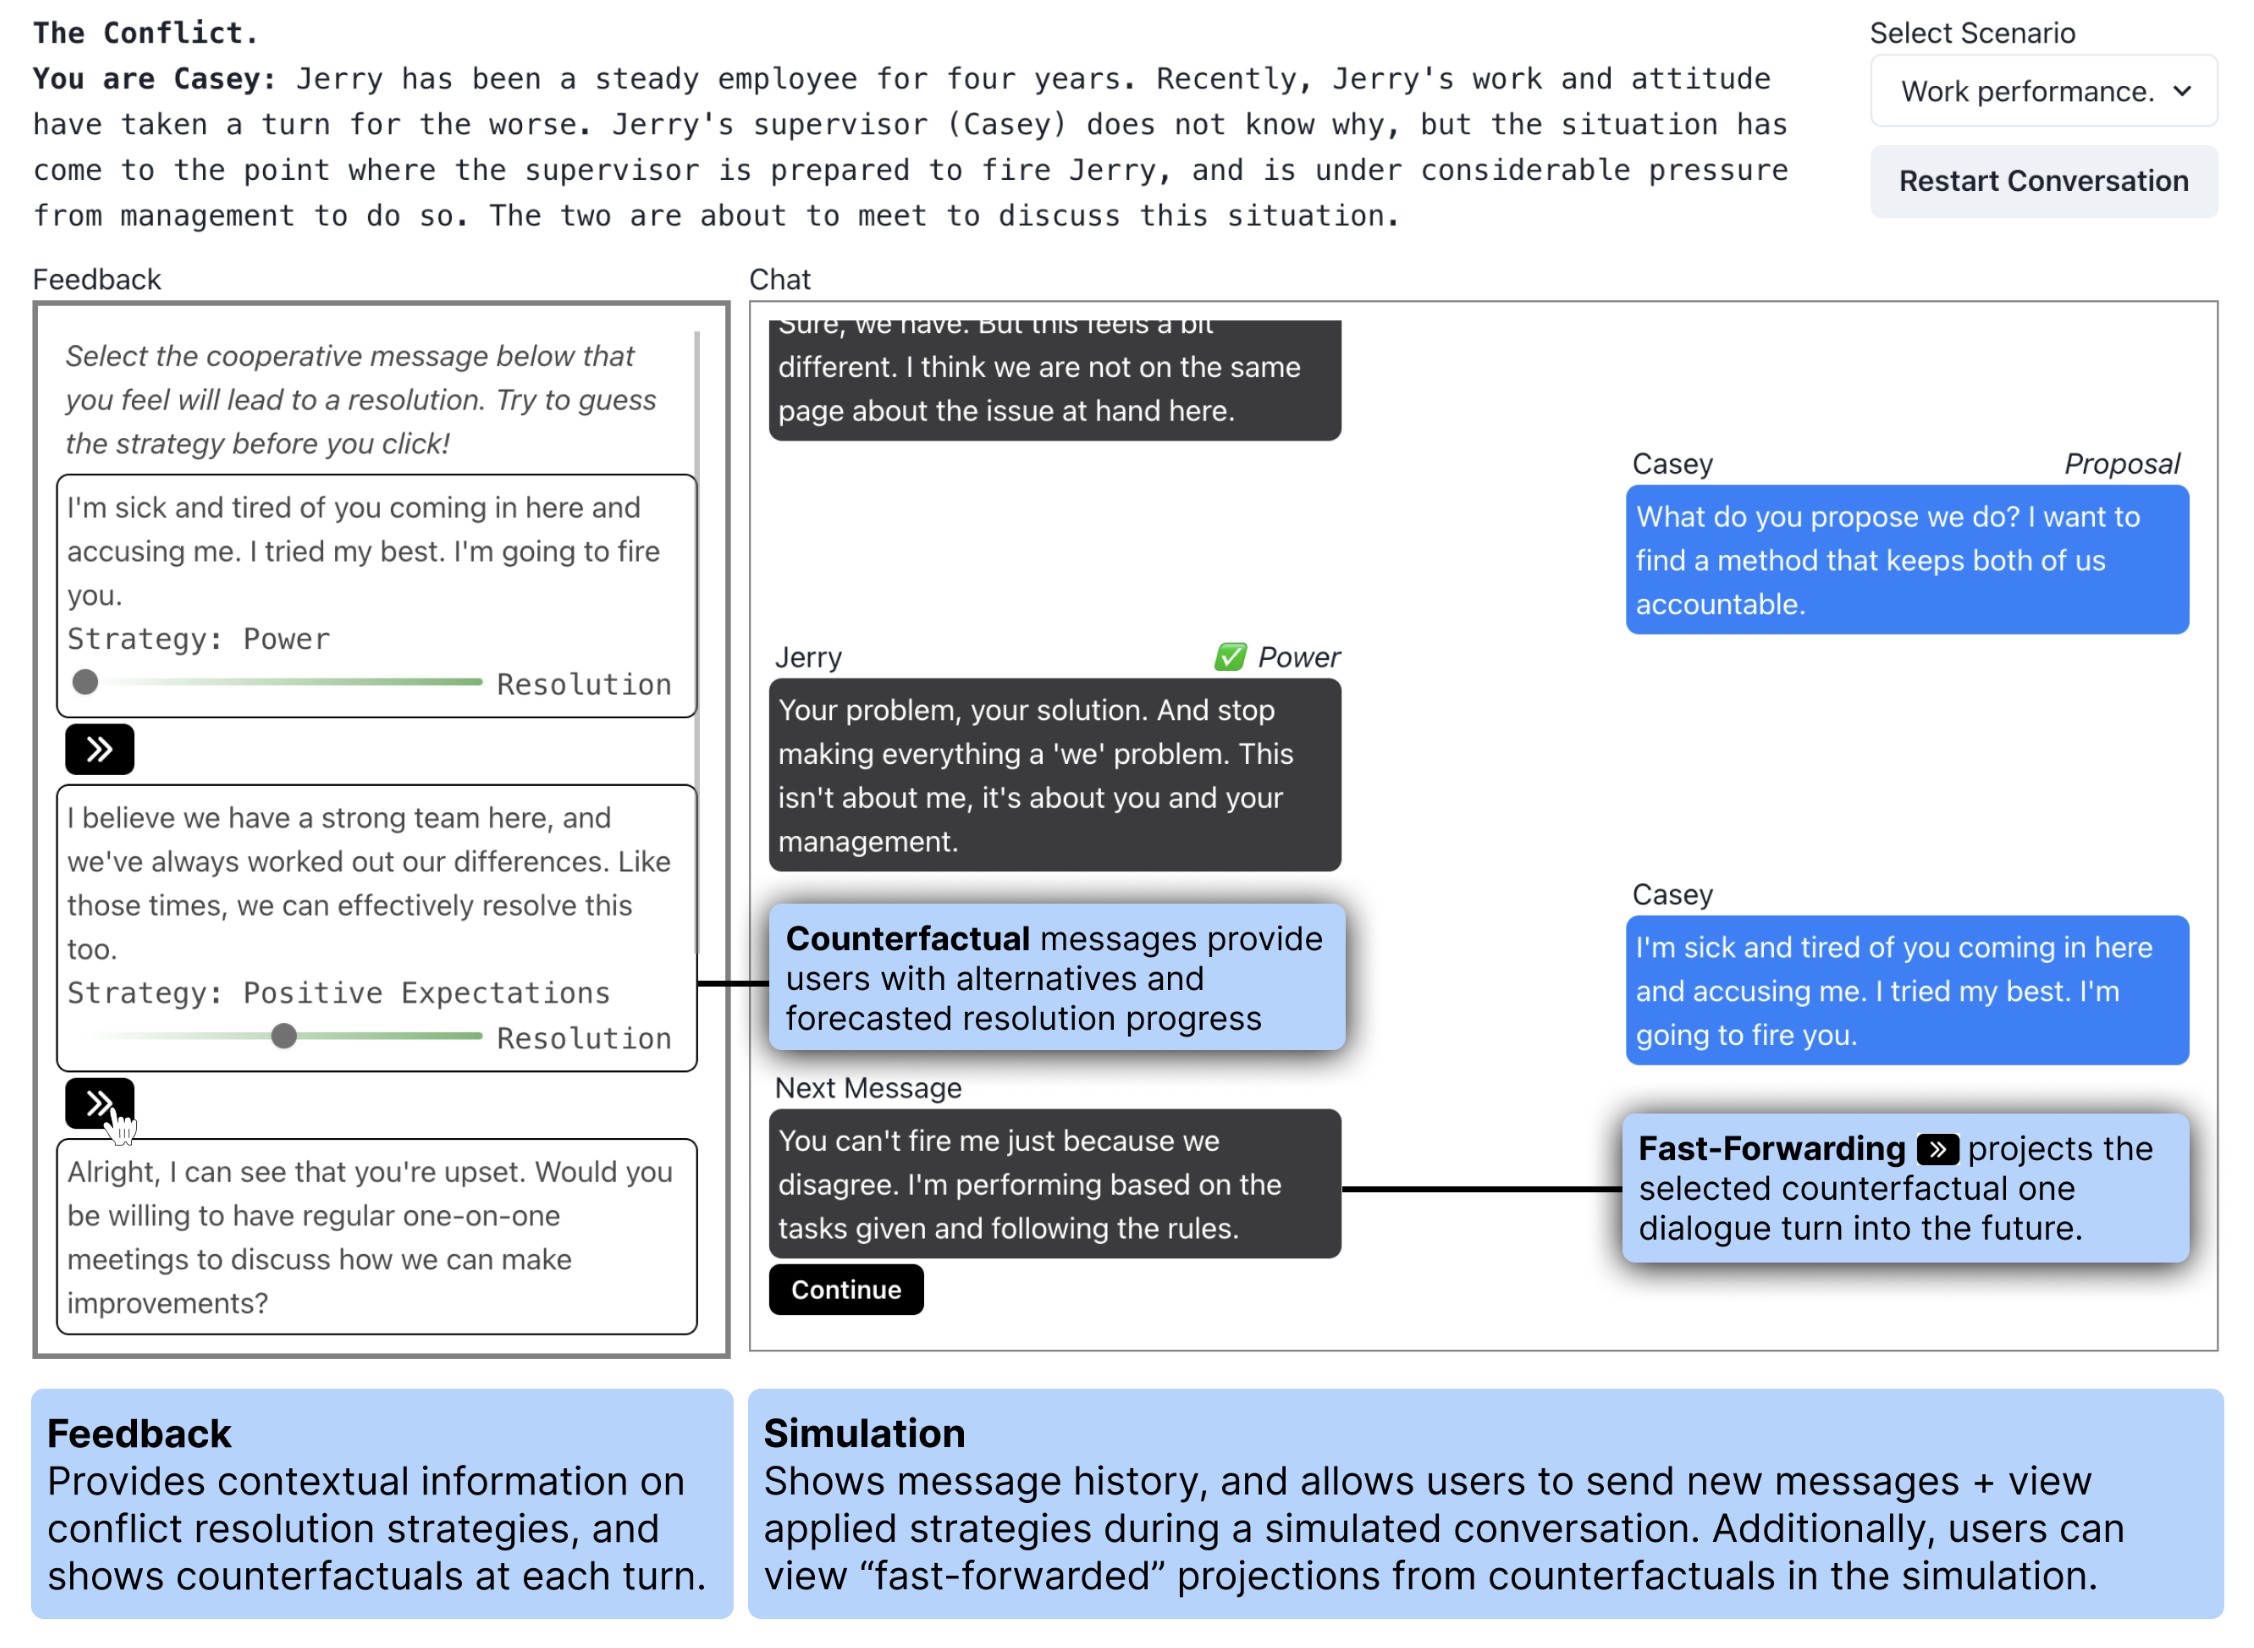
\includegraphics[width=\linewidth]{rehearsal.png}
        \end{column}
    \end{columns}
\end{frame}

\begin{frame}
    \frametitle{AI on My Shoulder (Swain, NEU-MS, CHI 2025)\footnote{\tiny Swain, V. (2024). \textit{AI on My Shoulder: Supporting Emotional Labor in Front-Office Roles with an LLM-based Empathetic Coworker} CHI 2025.}}
    \footnotesize
    \vspace{-0.2cm}
    \centering
    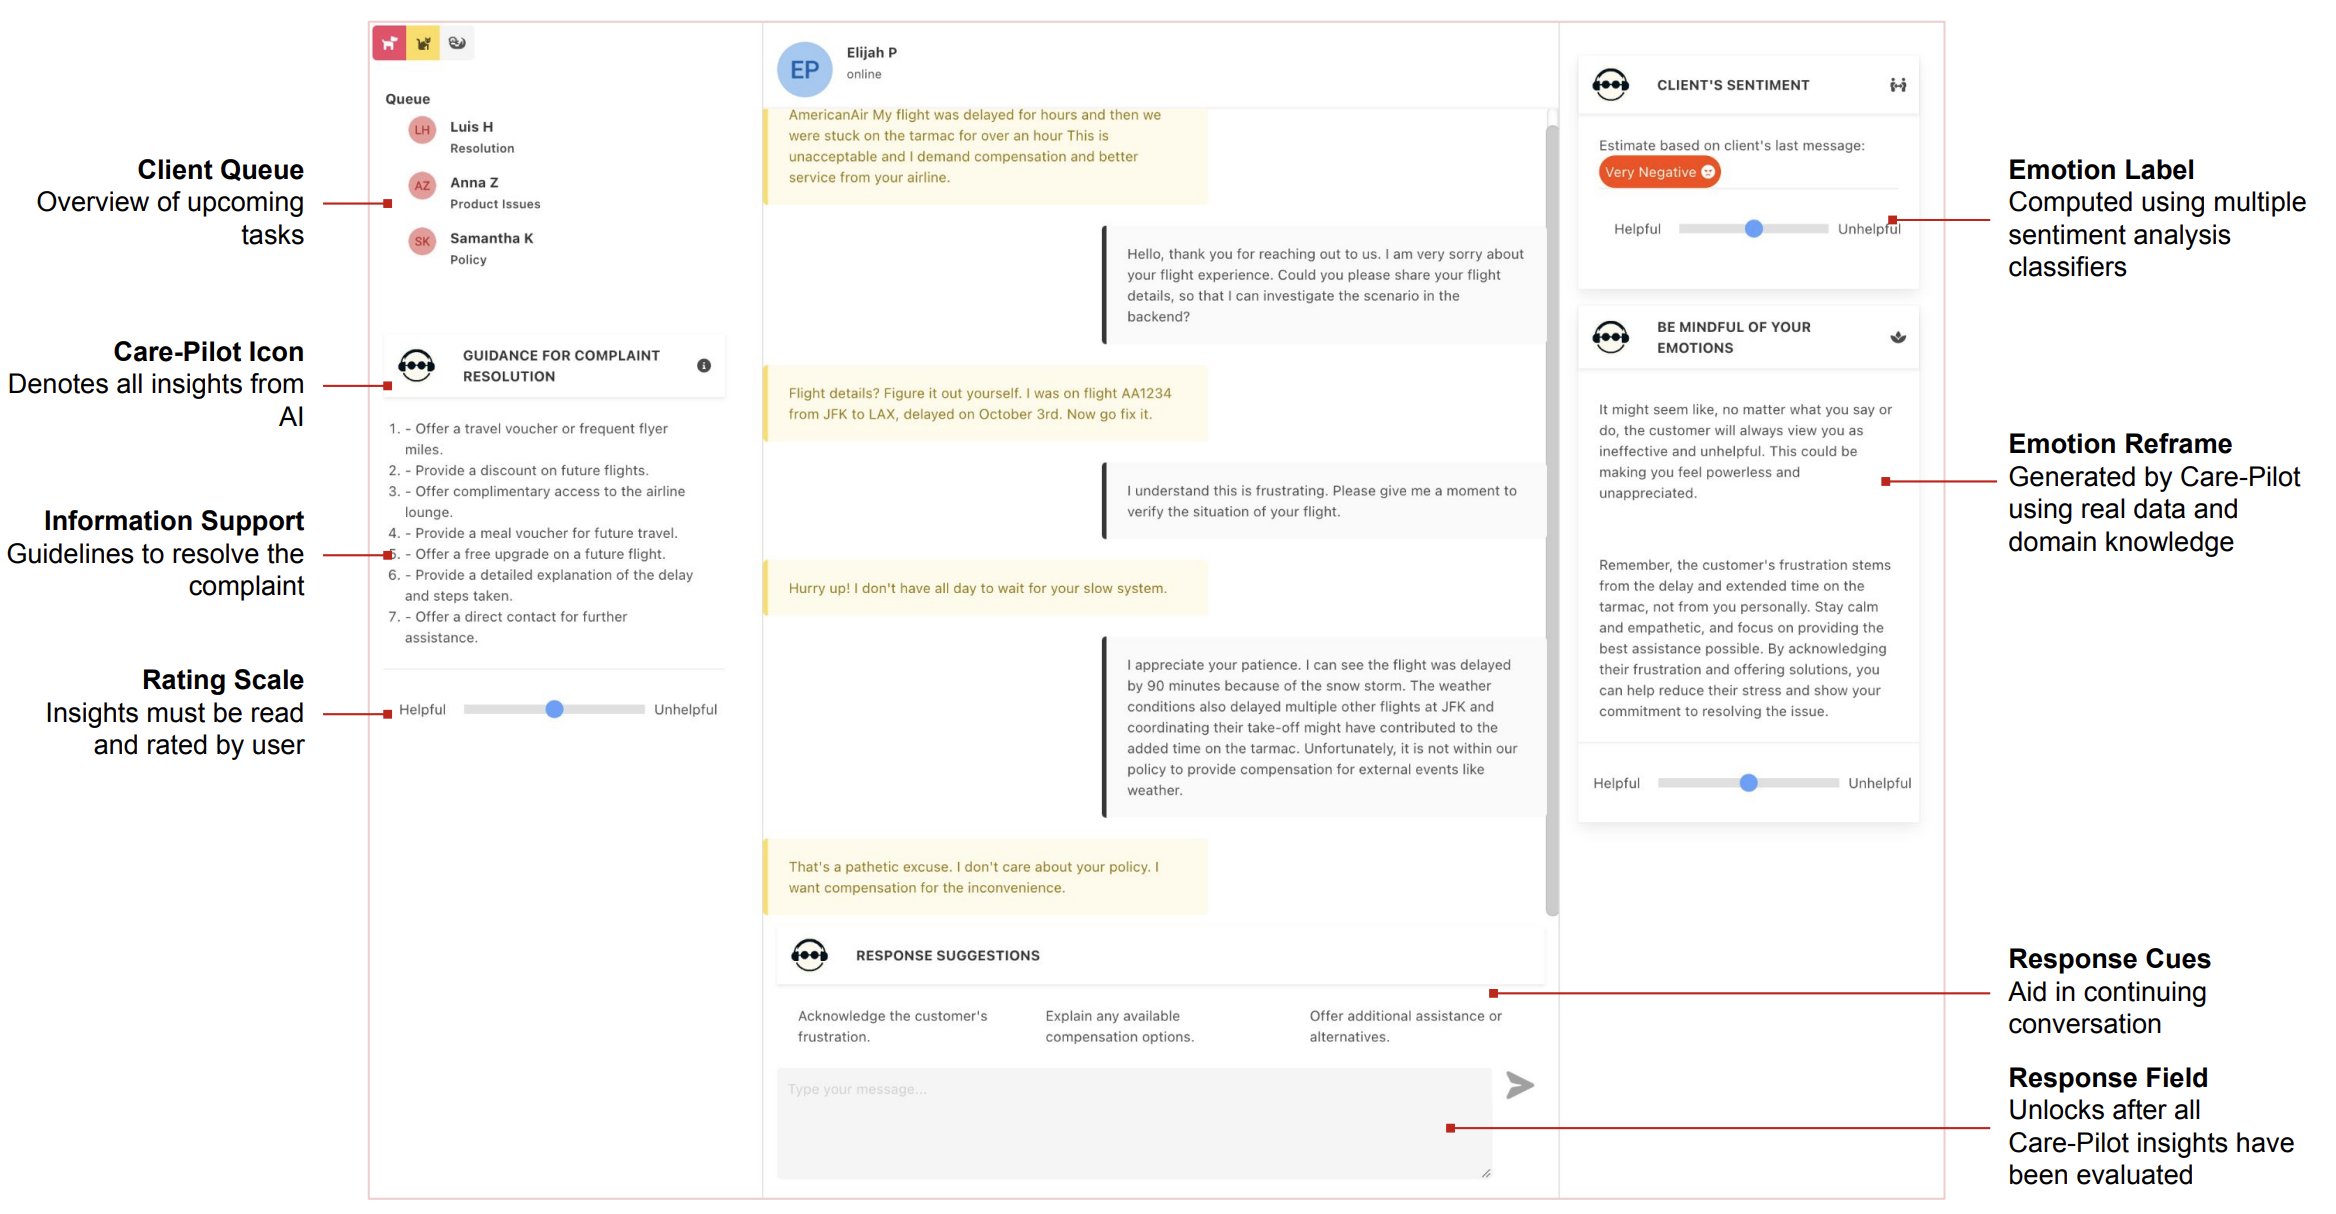
\includegraphics[width=0.85\linewidth]{aionmyshoulder5.png}
    \begin{columns}
        % Left column
        \begin{column}{1.0\textwidth}
        \vspace{-0.5em}
        \centering
        % 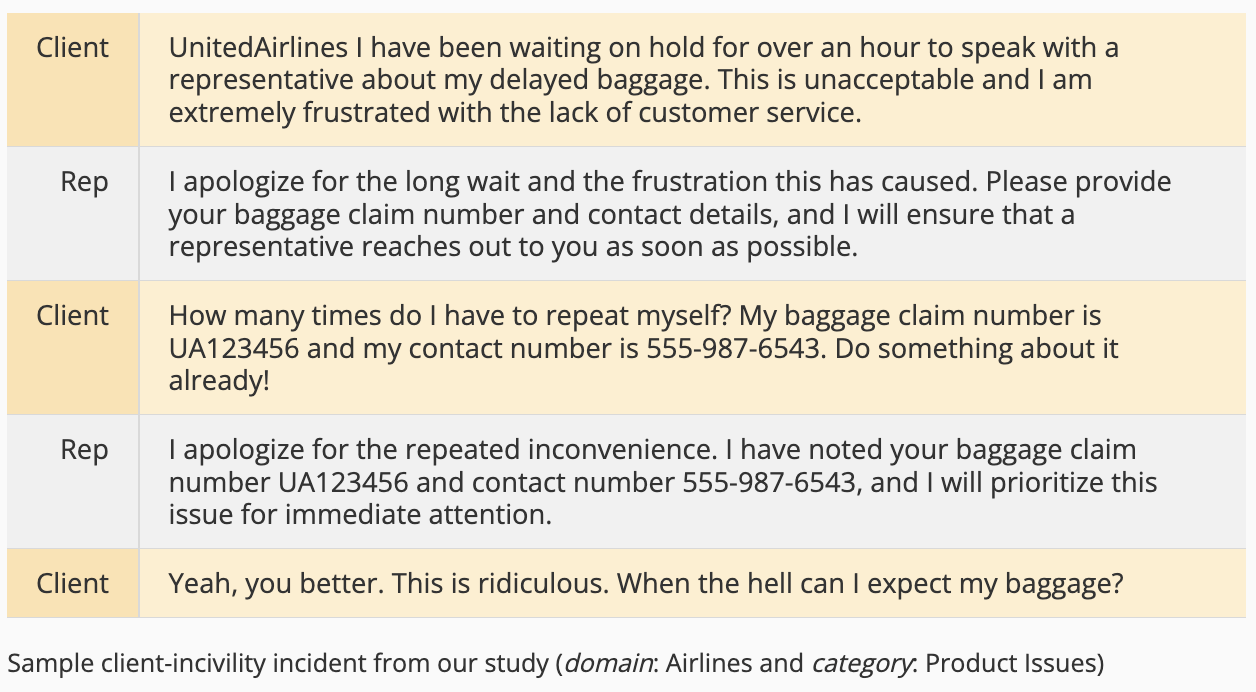
\includegraphics[width=0.65\linewidth]{aionmyshoulder4.png}
            \begin{itemize}
                \item \textbf{Goal}: To investigate how an LLM-based AI coworker can help Client-Service Representatives (CSRs) regulate their emotions in real-time
                % \item \textbf{System} Interactive system that uses LLM to help regulate CSRs 
                \item \url{https://www.youtube.com/watch?v=S4vPJ7_4l80}
            \end{itemize}
        \end{column}
        
        % Right column
        % \begin{column}{0.45\textwidth}
        %     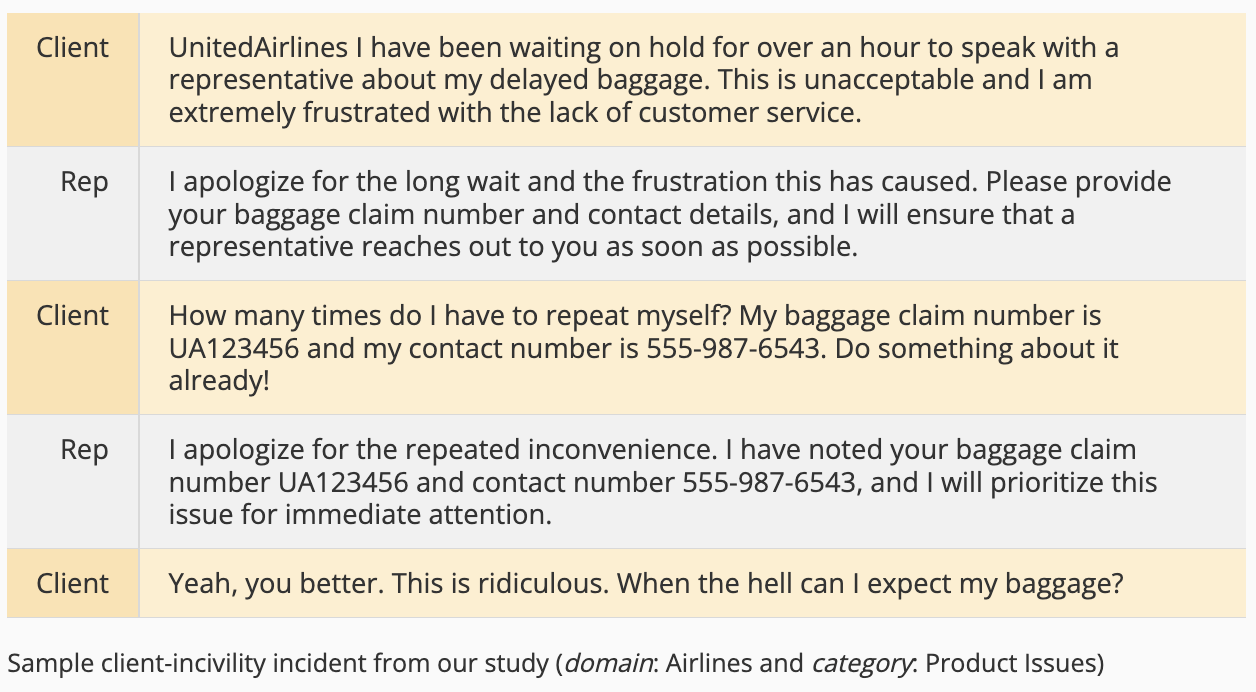
\includegraphics[width=\linewidth]{aionmyshoulder4.png}
        % \end{column}
    \end{columns}
\end{frame}

\begin{frame}
    \frametitle{AI on My Shoulder Conti ... (Swain, NEU-MS, CHI 2025)\footnote{\tiny Swain, V. (2024). \textit{AI on My Shoulder: Supporting Emotional Labor in Front-Office Roles with an LLM-based Empathetic Coworker} CHI 2025.}}
    \footnotesize
    \begin{columns}
        % Left column
        \begin{column}{0.55\textwidth}
        \vspace{-1.0em}
            \begin{itemize}
                \item \textbf{IVs}: Types of client interactions (Civil with informational support (IS) vs Uncivil with IS vs Uncivil with full Care-Pilot including informational, sentiment label, and emotional reframing panels)
                \item \textbf{DV}: Cognitive demands, cognitive resources, affect (pleasure and energy levels), helpfulness, perceptions of AI-mediated support, 
                \item \textbf{Participants}: 665 participants
                \item \textbf{Key Findings}: 
                \begin{itemize}
                \scriptsize
                \item Effective "in-the-moment" emotional regulation  
                \item Good on-task support and training tool 
                \item Lacks social connectedness and shared lived experience
            \end{itemize}
            \end{itemize}
        \end{column}
        
        % Right column
        \begin{column}{0.47\textwidth}
            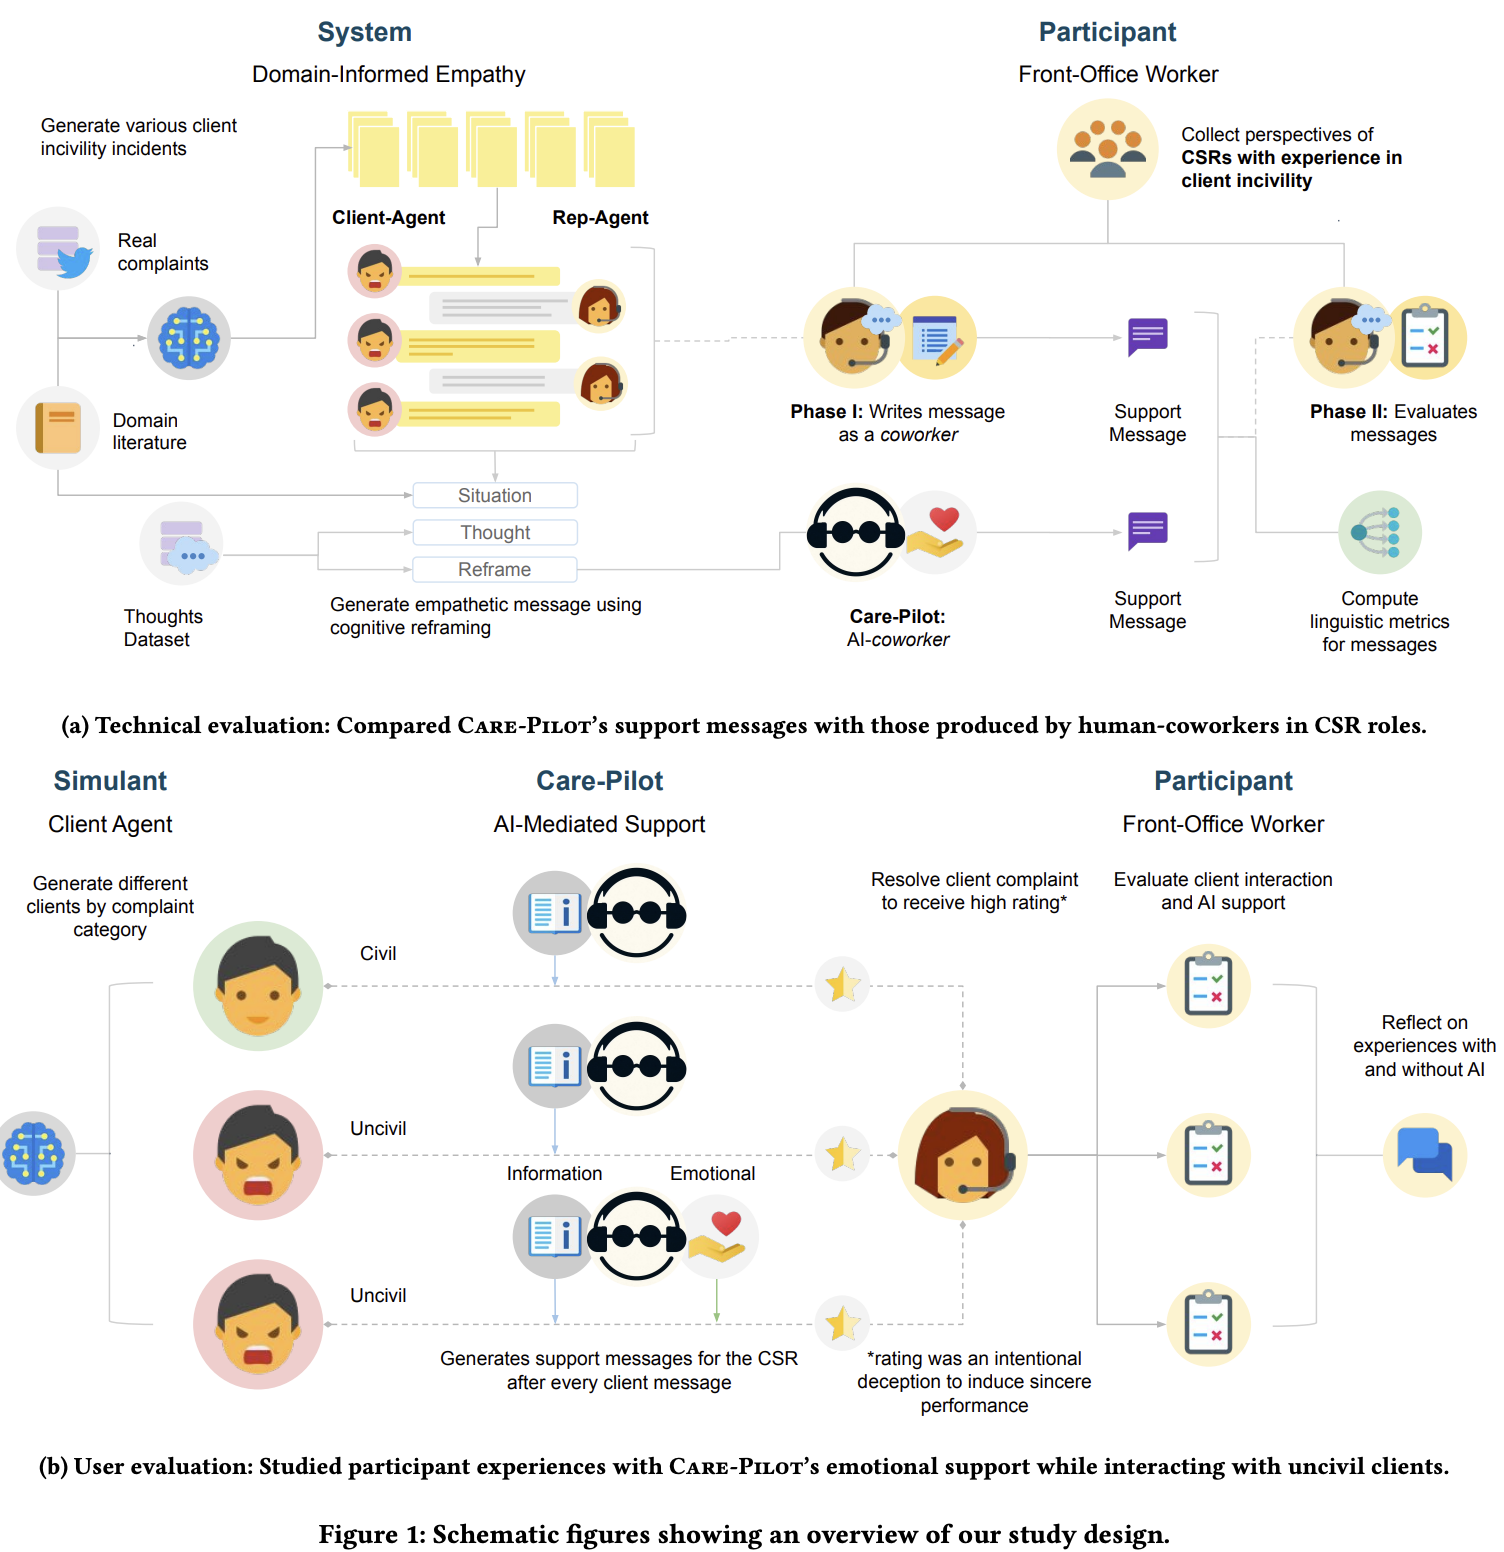
\includegraphics[width=\linewidth]{aionmyshoulder3.png}
        \end{column}
    \end{columns}
\end{frame}

\begin{frame}
    \frametitle{Generative and Malleable UI (Cao, CHI 2025)\footnote{\tiny Cao, Y. (2025). \textit{Generative and Malleable User Interfaces with Generative and Evolving Task-Driven Data Model} CHI 2025.}}
    \footnotesize
      % \centering
      % \includegraphics[width=0.85\textwidth]{HCI x AI/gen_mall_ui.png}
      % \vspace{-2.0em}
    \begin{columns}
        % Left column
        \begin{column}{0.5\textwidth}
            \vspace{-3.0em}
            \centering
            \includegraphics[width=0.85\textwidth]{HCI x AI/gen_mall_ui.png}
            \vspace{2.0em}
            \begin{itemize}
                \item \textbf{Problem}: Current UIs require users to piece together many applications to complete a single task
                \item \textbf {Goal}: To create generative and malleable UIs that dynamically adapts to user's diverse and evolving task
                \item \textbf{Task}: Participants are asked to complete 2 tasks of their choice 
                \item \url{https://www.youtube.com/watch?v=X3cf1U1dFGQ}
            \end{itemize}
        \end{column}
        
        % Right column
        \begin{column}{0.5\textwidth}
            % \vspace{0.25em}
            % \includegraphics[width=\textwidth]{HCI x AI/gen_mall_ui.png}
            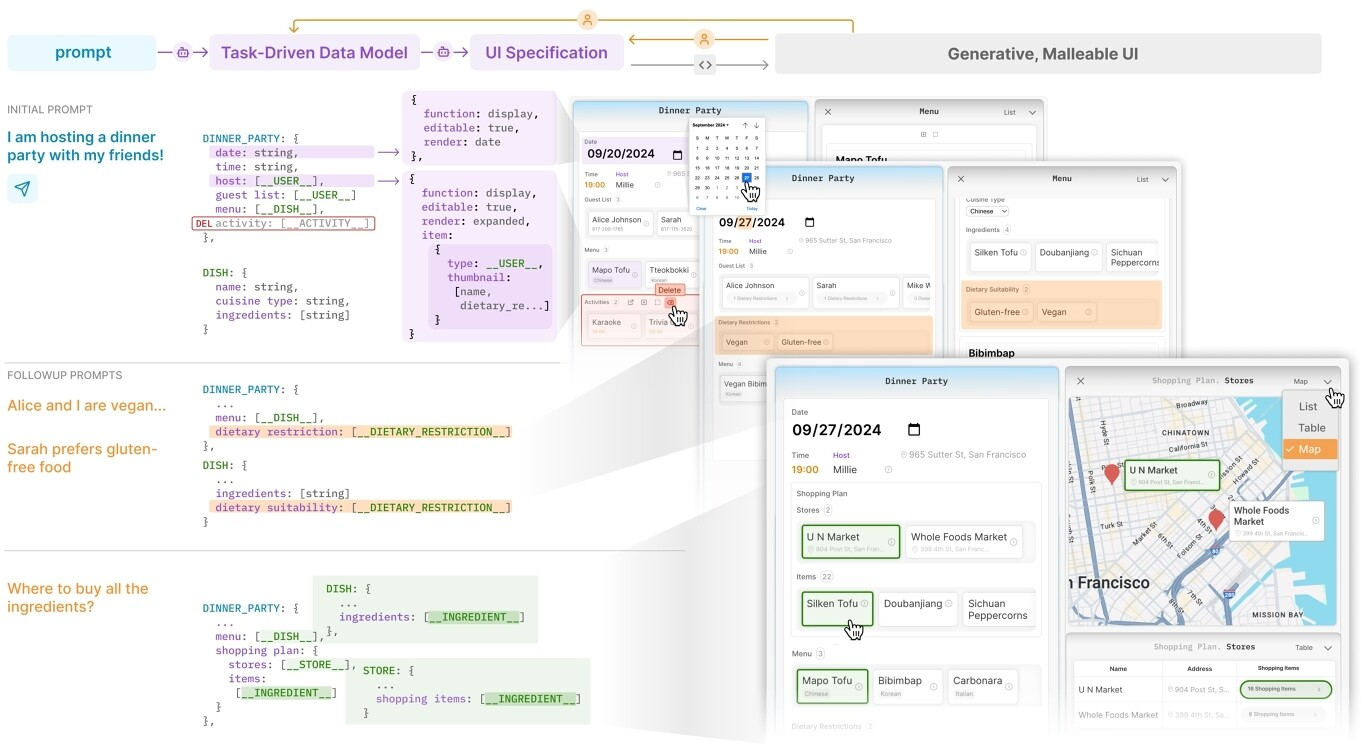
\includegraphics[width=\linewidth]{chi25-202-fig1.jpg}
            \vspace{-2.0em}
            \begin{itemize}
                \scriptsize

                \item \textbf{DV}: Information Relevance, Task Efficiency, Ease of use, Usefulness, Intuitiveness, Effective consumption of information
                \item \textbf{Participants}: 8 participants
                \item \textbf{Key Findings}: Effective info organization for task achievement, Sense of owner ship due to customizability and adaptation, Relying on continuous prompting for small changes is tedious
            \end{itemize}
        \end{column}
    \end{columns}
\end{frame}

\begin{frame}
    \frametitle{Generative Interfaces (Chen, SU, preprint 2025)\footnote{\tiny Chen, J. (2025). \textit{Generative Interfaces for Language Models} preprint 2025.}}
    \footnotesize
    {\centering
    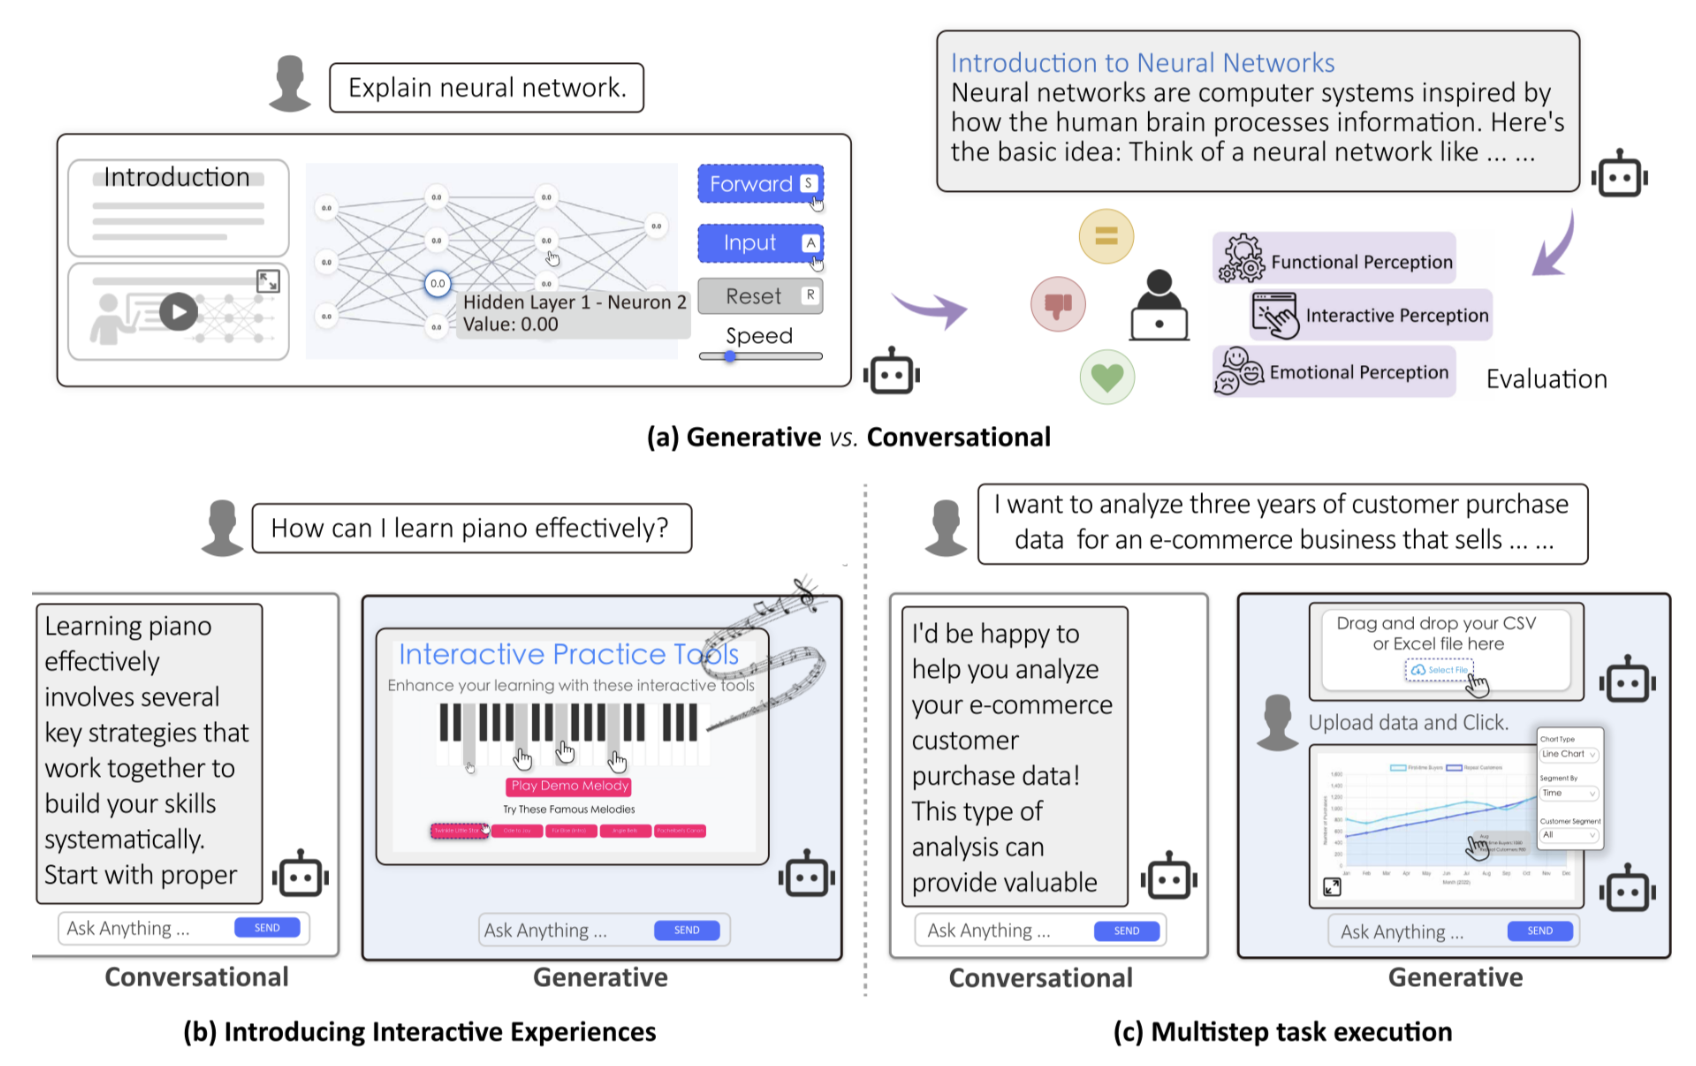
\includegraphics[width=0.75\linewidth]{generative_interface.png}\par}
    
    \textbf{Goal}: LLMs dynamically create adaptive and interative UIs to queries to better support complex exploratory and information-dense tasks
\end{frame}

\begin{frame}
    \frametitle{Generative Interfaces Conti ... (Chen, SU, preprint 2025)\footnote{\tiny Chen, J. (2025). \textit{Generative Interfaces for Language Models} preprint 2025.}}
    \footnotesize
    \begin{columns} %[t]
        % Left column
        \begin{column}{0.50\textwidth}
        \vspace{-1.0em}
            \begin{itemize}
                \item \textbf{IVs}: Type of UI (Conversational Interface vs Generative Interface) 
                \item \textbf{DV}: Functional Perception (query-interface consistency, task-efficiency) Interactive Perception (usability, learnability, information clarity), Emotional Perception (aesthetic and stylistic appeal (ASA), interactive experience satisfaction (IES))
                \item \textbf{Participants}: N/A. Three judgments were aggregated via majority vote to get a single final decision
                
            \end{itemize}
        \end{column}
        
        % Right column
        \begin{column}{0.50\textwidth}
            % {\tiny
            % 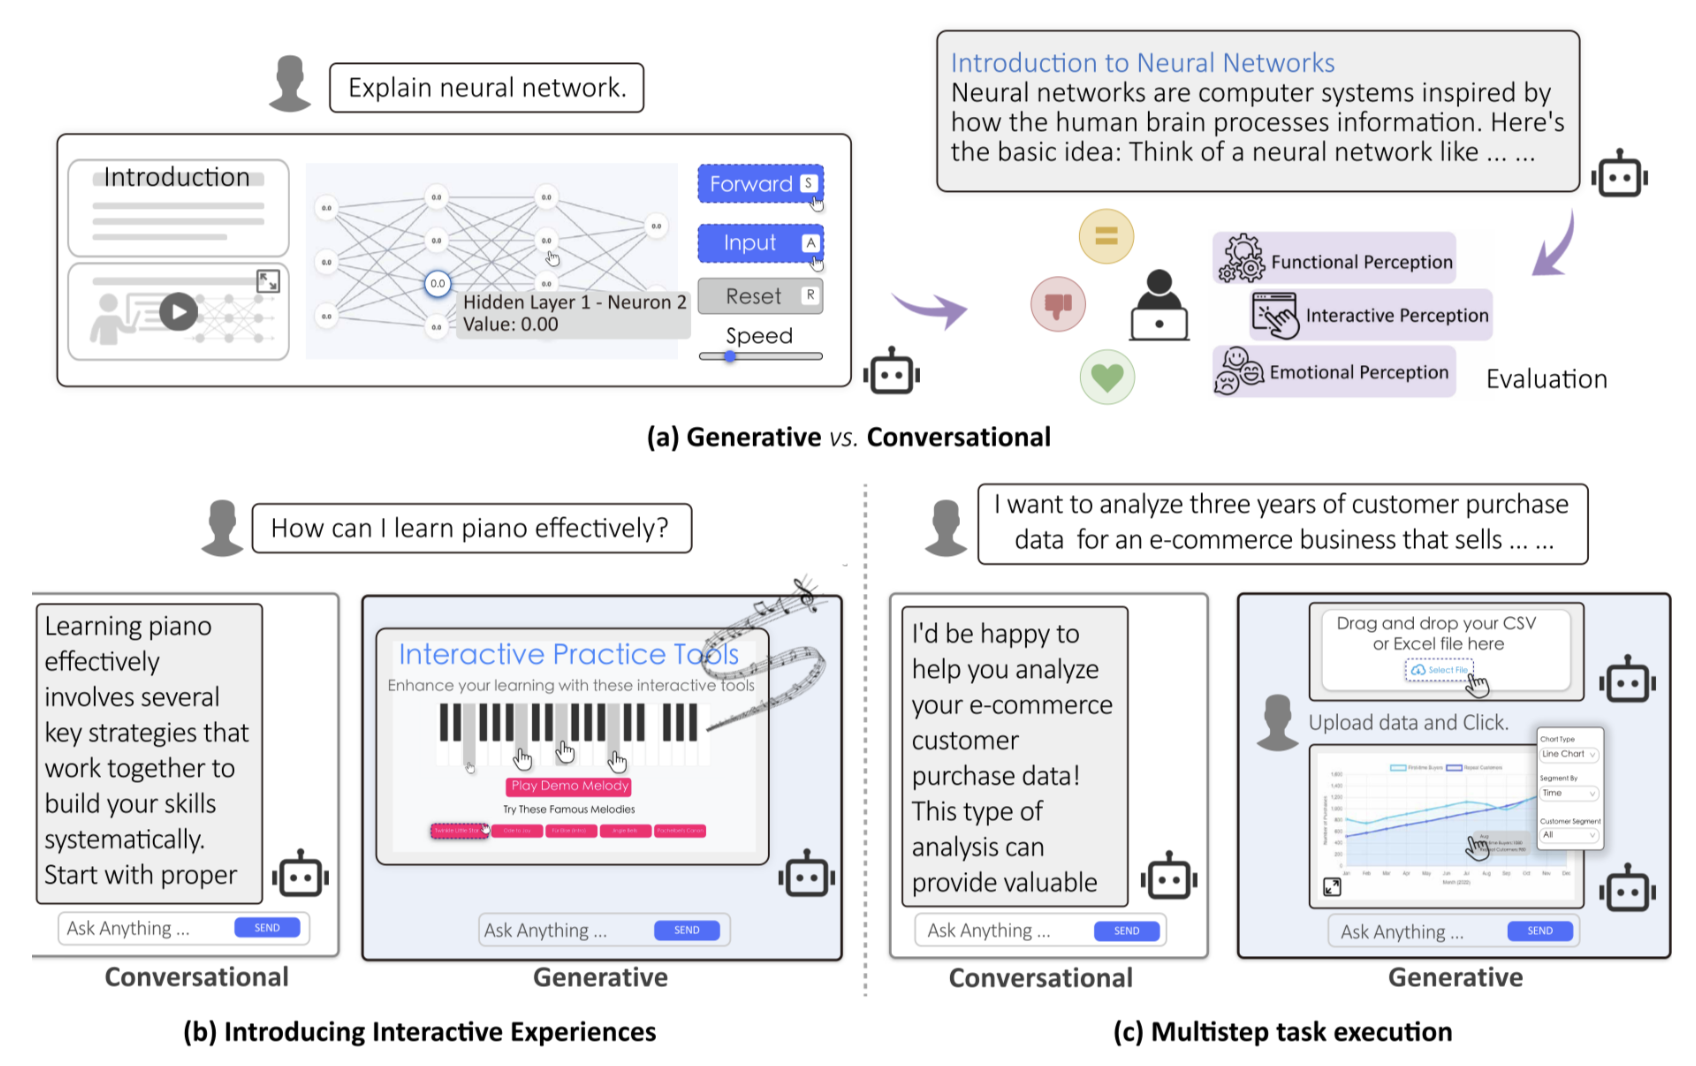
\includegraphics[width=\linewidth]{generative_interface.png}
            % \item \url{https://salt-nlp.github.io/generative_interfaces/}
            {\tiny
            \begin{itemize}
                \scriptsize
                \item \url{https://salt-nlp.github.io/generative_interfaces/}
                \item \textbf{Key Findings}:
                \begin{itemize}
                \scriptsize
                \item Human preferred GenUI in over 70 \% of cases.  
                \item Functional Perception: GenUI excelled in aligning with user queries and improving task efficiency.
                \item Interactive Perception: It was rated higher for usability, learnability, and clarity of information.
                \item Emotional Perception: The most significant gains were in ASA and IES.
                \end{itemize}
            \end{itemize}
        }
        \end{column}
    \end{columns}
\end{frame}


\begin{frame}
    \frametitle{Plan-then-Execute (He, Delft-Queensland, CHI 2025)\footnote{\tiny He, G. (2025). \textit{Plan-Then-Execute: An Empirical Study of User Trust and Team Performance When Using LLM Agents As A Daily Assistant} CHI 2025.}}
    \footnotesize
    \begin{columns}
        % Left column
        \begin{column}{0.60\textwidth}
        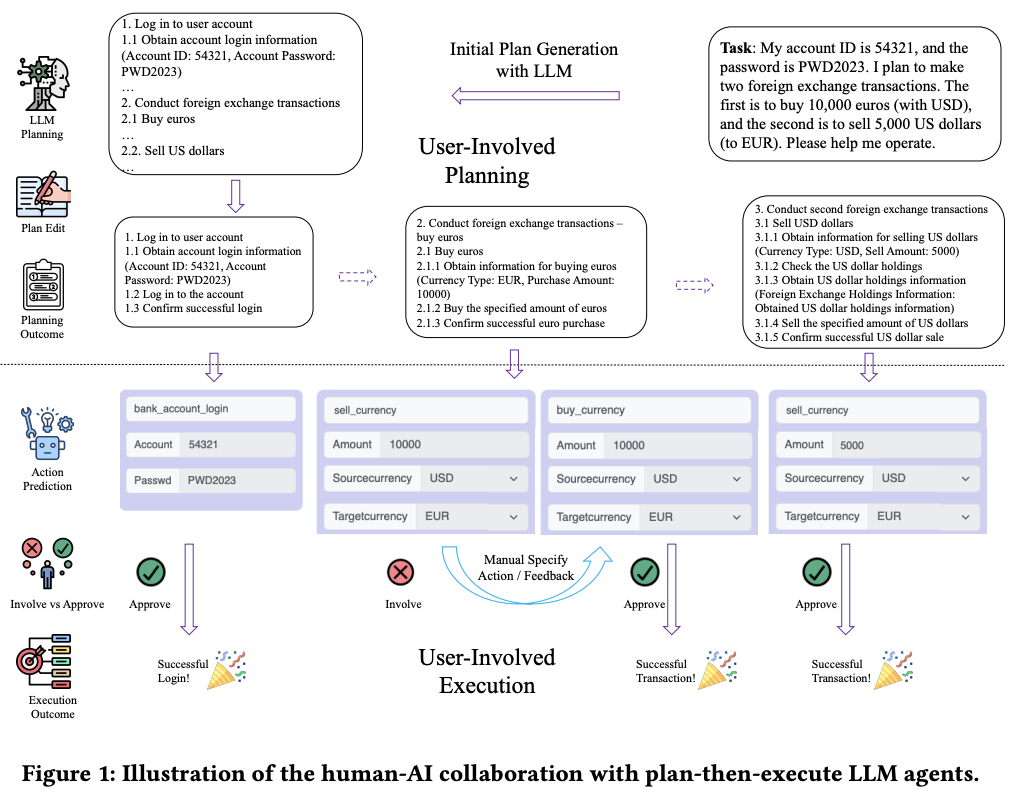
\includegraphics[width=\linewidth]{planexecute.png}
        \end{column}
        
        % Right column
        \begin{column}{0.40\textwidth}
            \vspace{-1.5em}
            \begin{itemize}
                \scriptsize
                \item \textbf{Problem}: LLM agents can produce plausible but incorrect plans or actions, creating risks, for high-stakes tasks like financial transactions 
                \item \textbf{Motivation}: How different levels of user involvement affect trust and team performance
            \end{itemize}
        \end{column}
    \end{columns}
\end{frame}

\begin{frame}
    \frametitle{Plan-then-Execute (He, Delft-Queensland, CHI 2025)\footnote{\tiny He, G. (2025). \textit{Plan-Then-Execute: An Empirical Study of User Trust and Team Performance When Using LLM Agents As A Daily Assistant} CHI 2025.}}
    \footnotesize
    \begin{columns}
        % Left column
        \begin{column}{0.50\textwidth}
        \vspace{-1.5em}
            \begin{itemize}
                \item \textbf{IVs}: Involvement (planning vs execution vs control), Tasks (high-risk e.g. payments vs low-risk e.g. booking flights)
                \item \textbf{DV}: Calibrated Trust (Planning and Execution), Task Performance (Plan quality, Action sequence accuracy, Execution accuracy)
                \item \textbf{Participants}: 248 participants.
                \item \url{https://www.youtube.com/watch?v=NdKXV68503M}
            \end{itemize}
        \end{column}
        
        % Right column
        \begin{column}{0.50\textwidth}
            \begin{itemize}
                % \scriptsize
                \item \textbf{Key Findings}:
                \begin{itemize}
                \scriptsize
                \item User planning did not significantly improve calibrated trust 
                \item Double edged sword: When initial plan was flawed, user involvement helped. But when initial plan was correct, user involvement made it worse and harmed the final performance. 
                \item Involvement increases cognitive load and lowers user confidence
                \end{itemize}
            \end{itemize}
        \end{column}
    \end{columns}
\end{frame}

\begin{frame}
    \frametitle{Towards Human-AI Deliberation (Ma, HKU, CHI 2025)\footnote{\tiny Ma, S. (2025). \textit{Towards Human-AI Deliberation: Design and Evaluation of LLM-Empowered Deliberative AI for AI-Assisted Decision-Making} CHI 2025.}}
    \footnotesize
      \centering
      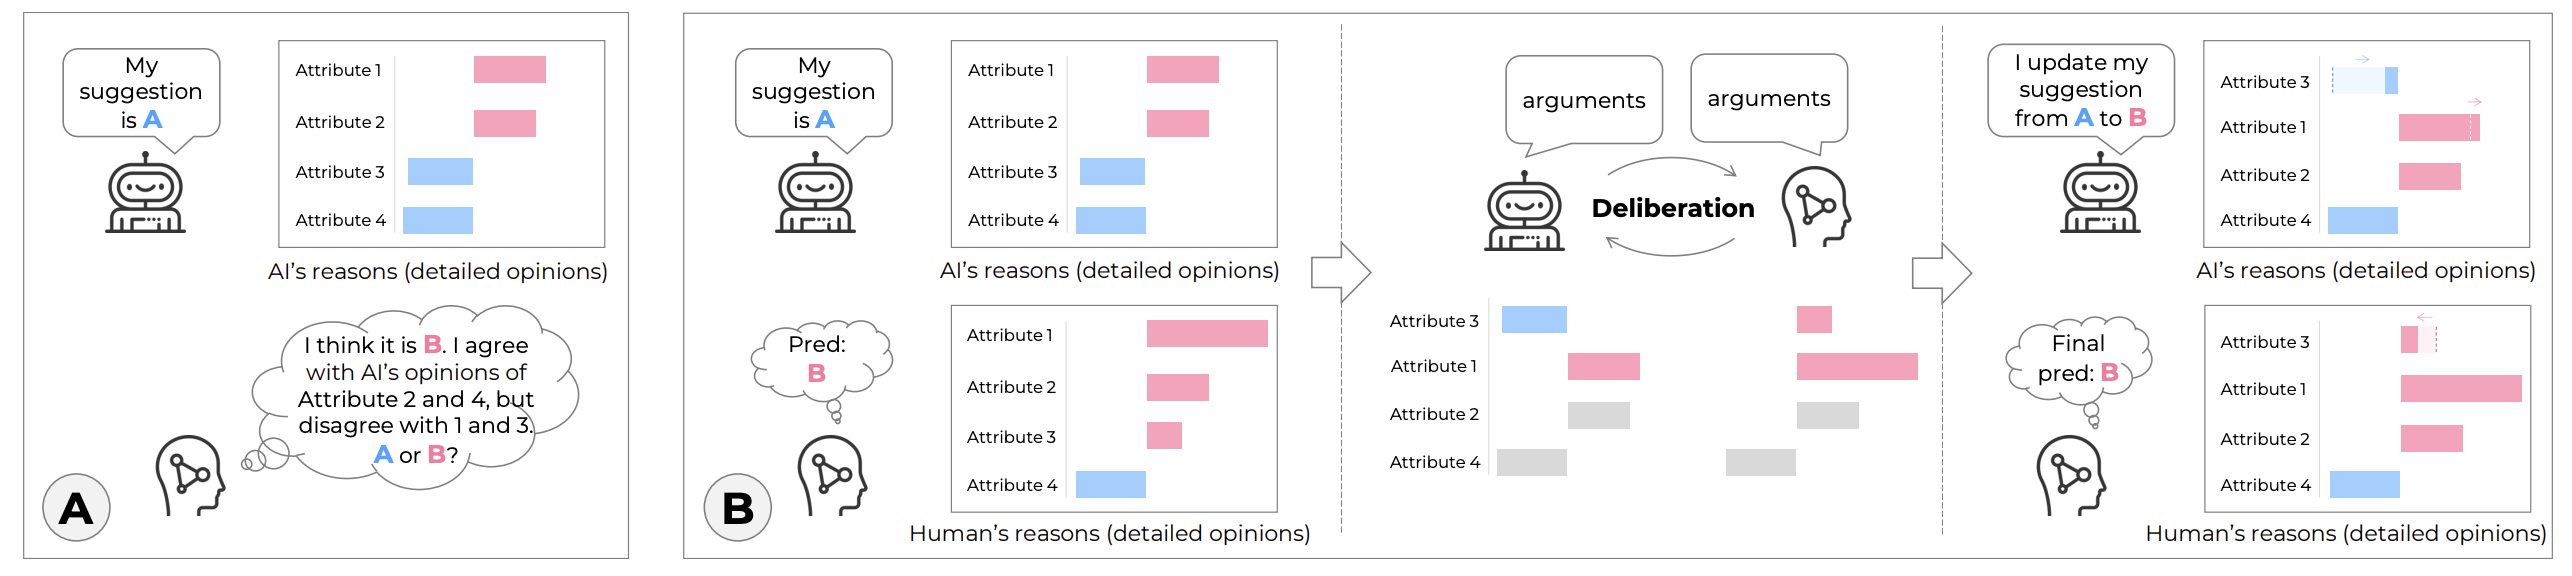
\includegraphics[width=0.85\textwidth]{humanaidecision.png}
      \vspace{-0.5em}
    \begin{columns}
        % Left column
        \begin{column}{0.53\textwidth}
            \begin{itemize}
                \item \textbf{Problem}: No analytical thinking with AI's suggestion: over/under-reliance on AI, Limited support to communicate disagreement or resolve conflict with AI: hinder effective collaboration
                \item \textbf{Goal}: Enable interactive, discussion-based process between humans-AI, especially when their opinions conflict 
                \item \textbf{IVs}: Type of assistance (Deliberative AI vs XAI vs Human)
                % \item \textbf{DV}: Task performance (Acc), Reliance on AI (agreement, switch fraction, over/under-reliance ratios), Behaviors (opinion change, freq of opinion change, time spent)
                % \item \textbf{Participants}: 153 participants
            \end{itemize}
        \end{column}
        
        % Right column
        \begin{column}{0.50\textwidth}
            % 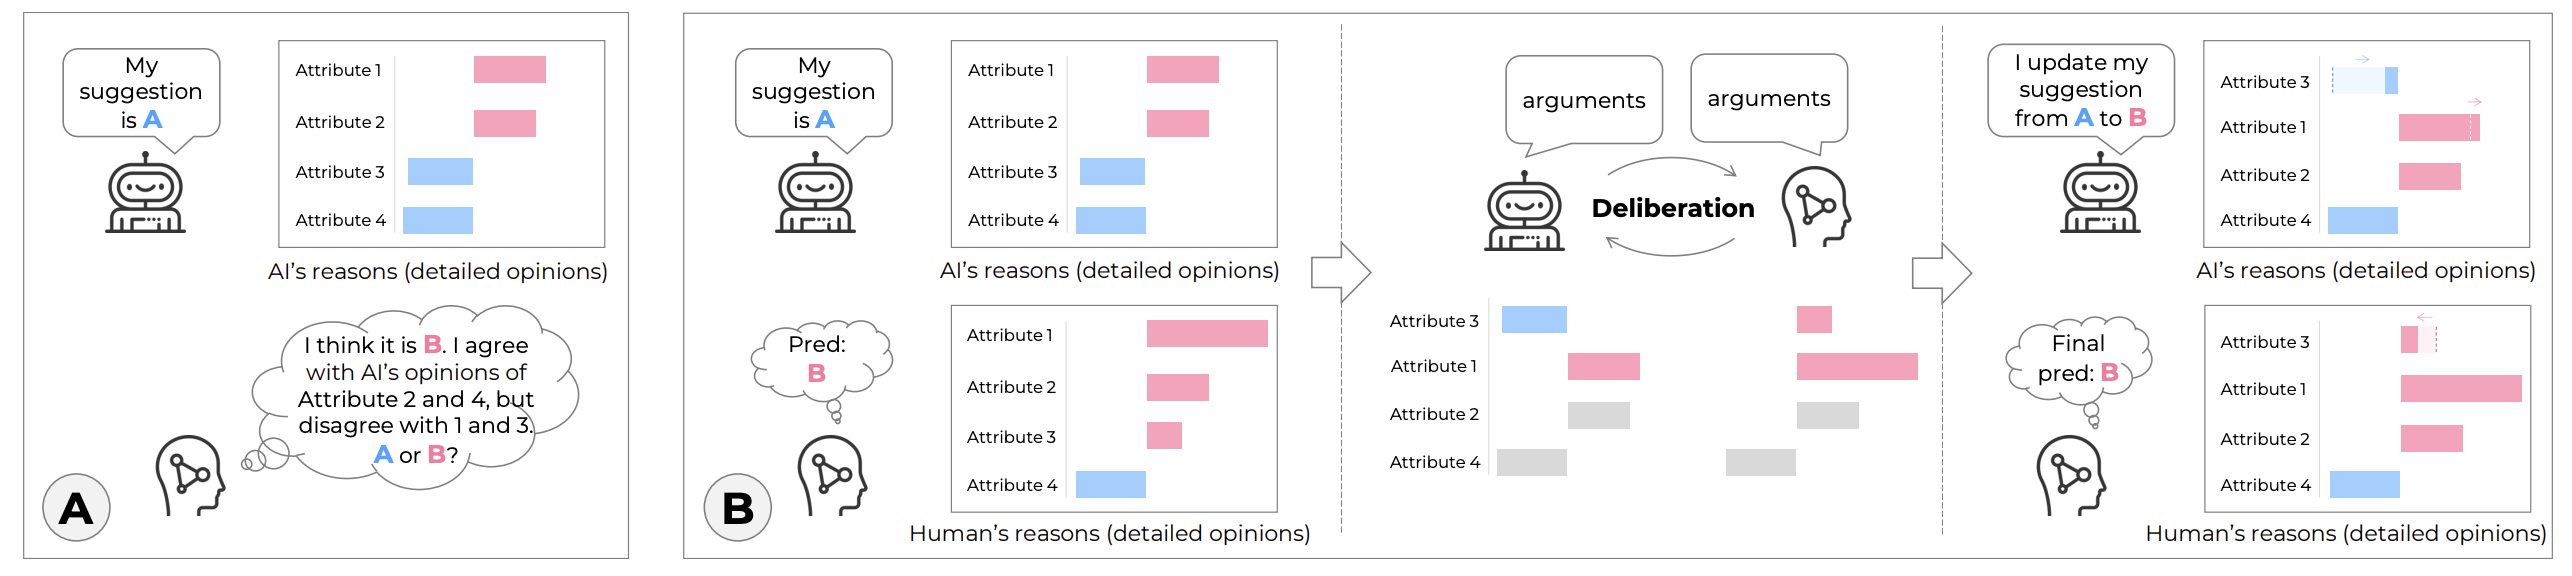
\includegraphics[width=\linewidth]{humanaidecision.png}
            \vspace{-0.25em}
            \begin{itemize}
                \scriptsize
                \item \textbf{DV}: Task performance (Acc), Reliance on AI (agreement, switch fraction, over/under-reliance ratios), Behaviors (opinion change, freq of opinion change, time spent)
                \item \textbf{Participants}: 153 participants
                \item \textbf{Key Findings}: 
                \begin{itemize}
                \item Improved decision accuracy by 8\%
                \item Reduce Over-reliance on Incorrect AI
                \item Encouraged more "system2" thinking 
                \end{itemize}
                \item \url{https://www.youtube.com/watch?v=GPwYyqGmkWc}
            \end{itemize}
            
        \end{column}
    \end{columns}
\end{frame}

\begin{frame}
    \frametitle{Beyond Text (Sun, Purdue, TMLR 2024)\footnote{\tiny Sun, X. (2024). \textit{Beyond Text: Utilizing Vocal Cues to Improve Decision
Making in LLMs for Robot Navigation Tasks} TMLR 2024.}}
    \footnotesize
    \begin{columns}
        % Left column
        \begin{column}{0.55\textwidth}
        \vspace{-1.5em}
            \begin{itemize}
                \item \textbf{Problem}: Human text of verbal instructions can be ambiguous or uncertain in robot navigation which are conveyed through vocal cues in Human-Robot Interaction
                \item \textbf{Goal}: Enable LLMs to analyze paralinguistic features alongside text transcriptions to better assess the trustworthiness of human guidance and improve the Robot's decision-making
                \item \textbf{IVs}: Type of info (text-only vs Text-COT-reasoning vs Text-VocalCues), LLMs( GPT3.5 vs GPT-3 vs Gemini-Pro)
                \item \textbf{DV}: Winning rate, confidence score, choice distribution, robustness to attack
                % \item \url{https://dl.acm.org/doi/full/10.1145/3706598.3713705}
            \end{itemize}
        \end{column}
        
        % Right column
        \begin{column}{0.47\textwidth}
            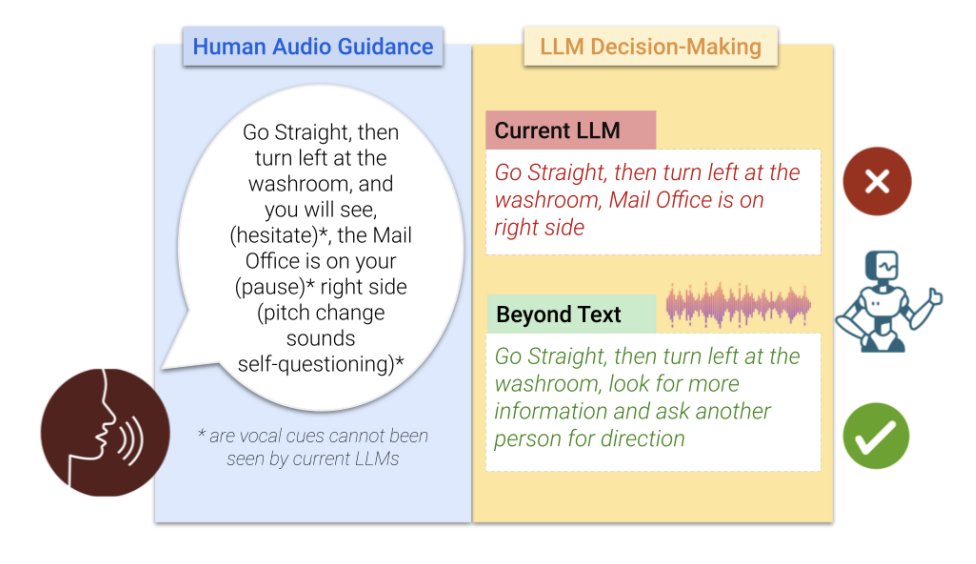
\includegraphics[width=\linewidth]{beyondtext.png}
            % \item \url{https://dl.acm.org/doi/full/10.1145/3706598.3713705}
            \begin{itemize}
                \vspace{-1.5em}
                \scriptsize
                \item \textbf{Key Findings}: 
                \begin{itemize}
                \scriptsize
                \item Higher winning rate and confidence
                \item LLMs shift from "blindly following" to "Handling Uncertainty"
                \end{itemize}
                % \item With vocal cues analysis
            \end{itemize}
        \end{column}
    \end{columns}
\end{frame}


%-----------------------------------------------

\section{Large-scale surveys / systematic review}

\begin{frame}
    \frametitle{Critical thinking (Lee et al., CMU and Microsoft, CHI 2025)\footnote{\tiny Lee et al. (2025). \textit{The Impact of Generative AI on Critical Thinking: Self-Reported Reductions in Cognitive Effort and Confidence Effects From a Survey of Knowledge Workers}}}
    \begin{itemize}
        \item \textbf{Large-scale survey study - 319 participants}: Each was asked to give 3 detailed examples of how they actually used a GenAI tool in their work: One \textbf{Creation} task (e.g., writing, designing, generating code). One \textbf{Information} task (e.g., searching, summarizing, analyzing data). One \textbf{Advice} task (e.g., getting feedback, validation, or guidance).
        \item Rated their examples on task types (the 3 categories), confidence ratings, did they use critical thinking, how much effort based on bloom's taxonomy, etc.
        \item Critical thinking depends on \textbf{self-confidence}, \textbf{motivation}, and \textbf{how much stake} is that task.
        \item Task type don't really matters
    \end{itemize}
\end{frame}

\begin{frame}
    \frametitle{Legal Advice (Seabrooke \& Clos, U. Southampthon, CHI 2025)\footnote{\tiny Seabrooke, T., \& Clos, J. (2025). \textit{Objection Overruled! Lay People Can Distinguish Large Language Model-Generated Legal Advice.}}}
    \begin{itemize}
        \item \textbf{Three experiments with 288 participants}: Lay people were asked to evaluate legal advice generated either by humans or large language models (LLMs). 
        \item Participants judged the advice for \textbf{quality, trustworthiness, and usefulness}, and were asked whether they would act on the advice.
        \item \textbf{Key finding 1}: Participants could distinguish LLM-generated advice from human advice.
        \item \textbf{Key finding 2}: Despite recognizing LLM-generated advice, participants were often \textbf{more willing to act} on it than on human-generated advice.
        \item \textbf{Implication}: AI can influence decision-making in legal contexts even when users know the advice is machine-generated, raising questions about \textbf{trust, reliance, and ethical use} of LLMs.
    \end{itemize}
\end{frame}

\begin{frame}
    \frametitle{Older Adults (Huang et al., U. California, CHI 2025)\footnote{\tiny Huang, Y., Zhou, Q., \& Piper, A. M. (2025). \textit{Designing Conversational AI for Aging: A Systematic Review of Older Adults' Perceptions and Needs.} CHI 2025.}}
    \scriptsize
    \begin{itemize}
        \item \textbf{Goal}: Understand what older adults want and need from chatbots or voice assistants.
        \item \textbf{Method}: Review of previous research on conversational AI for aging populations.
        \item \textbf{Important Insights}:
        \begin{itemize}
            \scriptsize
            \item \textbf{Empathy matters a lot}: Older adults prefer AI that feels understanding and “human-like,” not just functional.
            \item \textbf{Privacy is crucial}: They worry about who sees their info and want clear control over their data.
            \item \textbf{Ease of use is more than big buttons}: Voice input, clear instructions, and accessible design are key.
            \item \textbf{Social support}: AI can reduce loneliness but should not replace human contact.
            \item \textbf{Personalization helps engagement}: Tailoring responses to their preferences makes AI feel more useful and friendly.
        \end{itemize}
        \item \textbf{Design Tips}:
        \begin{itemize}
            \scriptsize
            \item AI should notice emotions and respond empathetically.
            \item Give simple, clear instructions and feedback.
            \item Let users control what the AI remembers or shares.
            \item Include features for people with vision, hearing, or cognitive challenges.
        \end{itemize}
    \end{itemize}
\end{frame}

\section{Experimental studies}

\begin{frame}
    \frametitle{False Memories (Pataranutaporn, MIT Media Lab, CHI 2025)\footnote{\tiny Pataranutaporn, P. (2025). \textit{AI-Edited Images and Videos Can Implant False Memories and Distort Recollection.} CHI 2025.}}
    \footnotesize
    \begin{columns}
        % Left column
        \begin{column}{0.55\textwidth}
            \begin{itemize}
                \item \textbf{Motivation}: Examine whether AI-edited images/videos can distort memory or create false memories.
                \item \textbf{Task}: Participants viewed media (images/videos) and later recalled specific details.
                \item \textbf{IVs}: Type of media (original vs AI-edited), subtlety of edits (obvious vs subtle).  
                \item \textbf{DV}: Number of false memories, accuracy of recalled details.  
                \item \textbf{Participants}: 120 participants.
            \end{itemize}
        \end{column}
        
        % Right column
        \begin{column}{0.45\textwidth}
            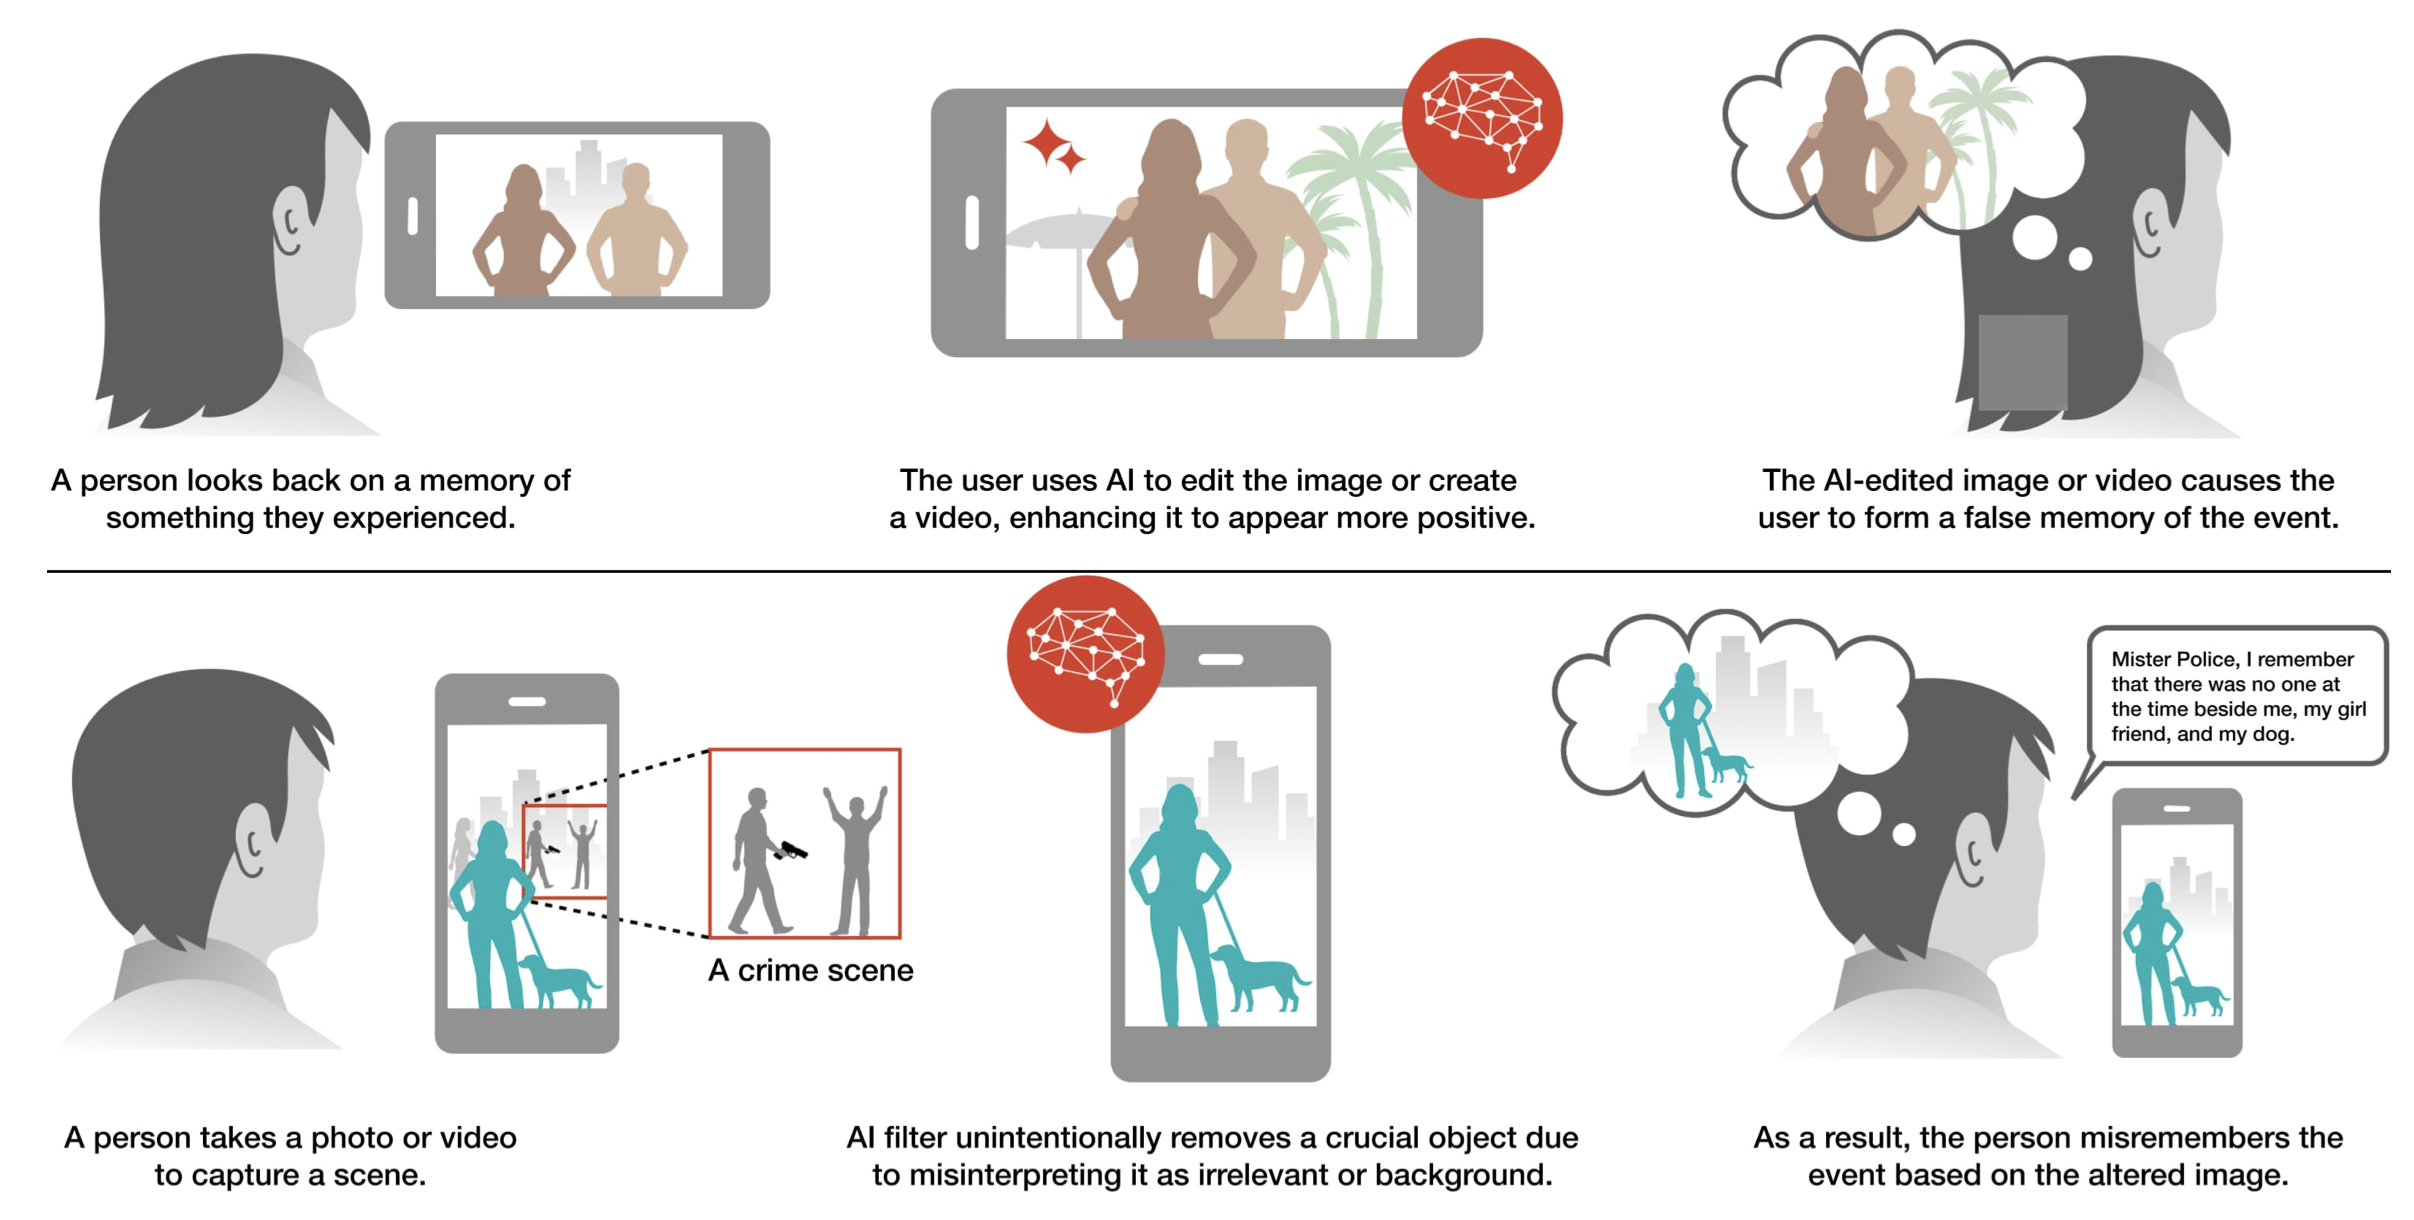
\includegraphics[width=\linewidth]{falsemem.png}
            \item \url{https://youtu.be/PiH066tA8aA}
            \begin{itemize}
                \scriptsize
                \item AI-edited media caused more false memories than original content.  
                \item Subtle edits were sometimes more deceptive than obvious ones.  
                \item Implication: Critical media literacy is important when interacting with AI-generated content.
            \end{itemize}
        \end{column}
    \end{columns}
\end{frame}

\begin{frame}
    \frametitle{Confirmation Bias (Rosbach et al., THI Germany, CHI 2025)\footnote{\tiny Rosbach, E., Ammeling, J., Krügel, S., et al. (2025). \textit{When Two Wrongs Don’t Make a Right – Examining Confirmation Bias and the Role of Time Pressure During Human-AI Collaboration in Computational Pathology.} CHI 2025.}}
    \scriptsize
    \begin{columns}
        \begin{column}{0.55\textwidth}
            \begin{itemize}
                \item Study how AI suggestions affect confirmation bias and how time pressure changes this effect.
                \item \textbf{Task}: 28 pathologists estimated tumor cell percentages from images by first estimating, wait for 2 weeks, then see AI suggestions, then make final estimations
                \item \textbf{IVs}: AI suggestion (matches or contradicts human bias), time pressure (high/low)
                \item \textbf{DV}: Accuracy and amount of bias (difference from true tumor percentage)
                \item When AI \textbf{agreed with a pathologist’s mistake}, it made the mistake \textbf{worse} (confirmation bias increased).  When AI disagree, pathologist tends to correct to more accurate answer.
            \end{itemize}
        \end{column}
        \begin{column}{0.45\textwidth}
            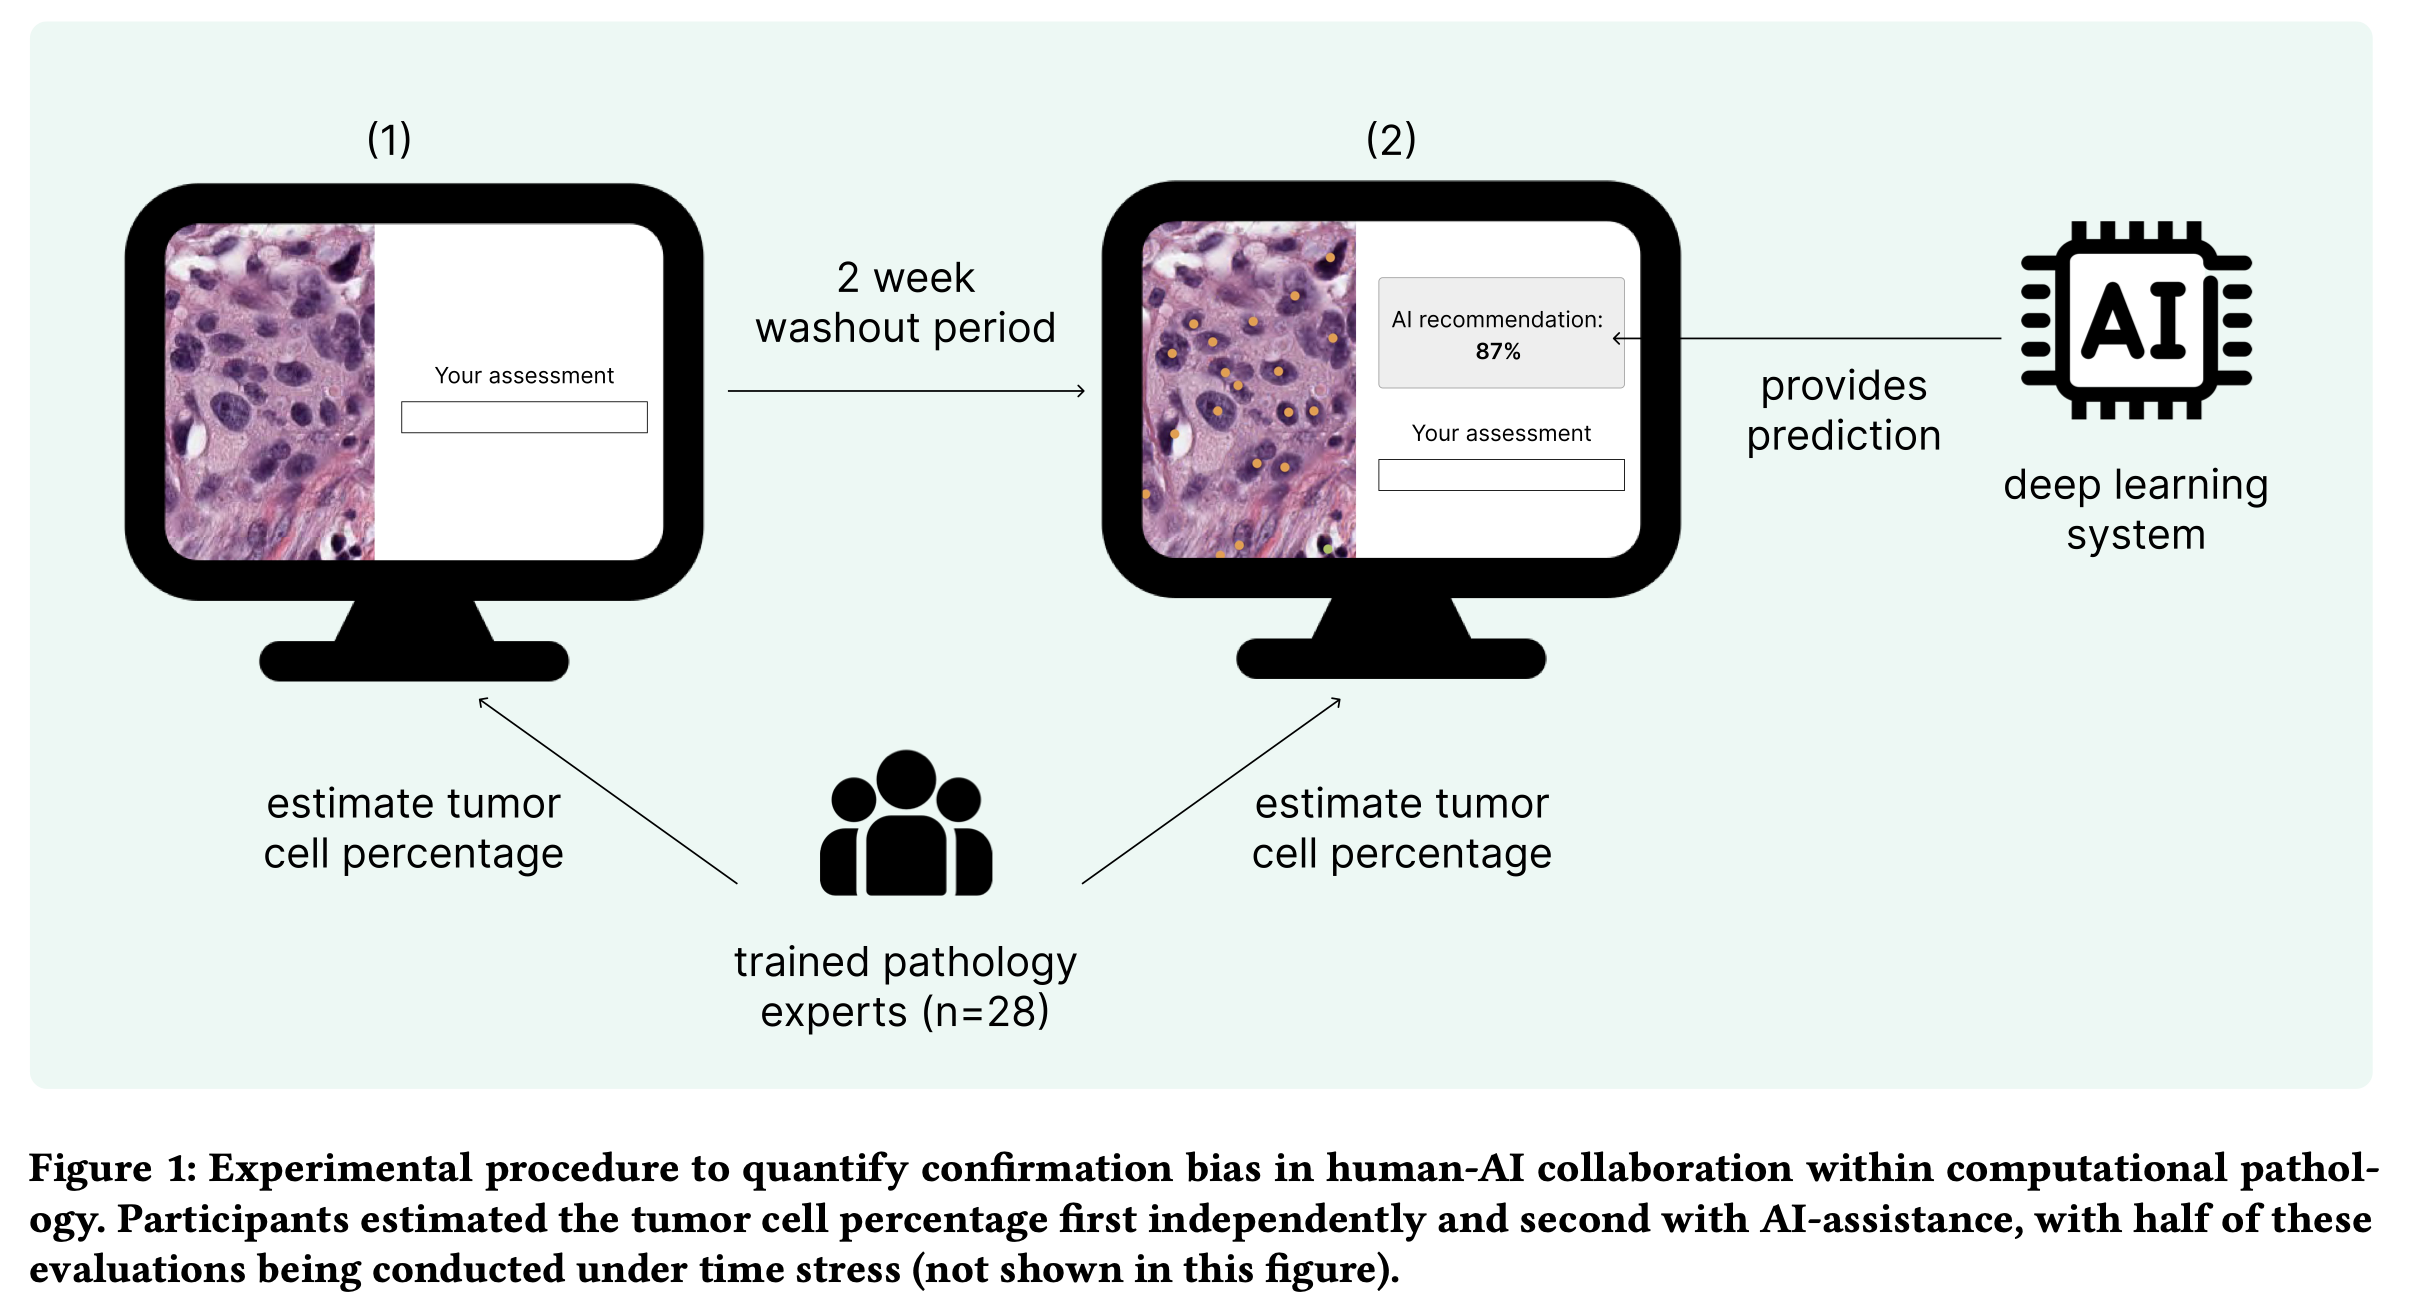
\includegraphics[width=\linewidth]{conbias.png}
            \item \url{https://www.youtube.com/shorts/Iibmg3ohn34}
            \item Working under \textbf{time pressure} made pathologists rely less on AI, reducing bias—but they made \textbf{more general mistakes}
        \end{column}
    \end{columns}
\end{frame}

\begin{frame}
    \frametitle{Proactive Chatbots (Liu et al., U. California, CHI 2025)\footnote{\tiny Liu, X., et al. (2025). \textit{Proactive Conversational Agents with Inner Thoughts.} CHI 2025.}}
    \scriptsize
    \begin{columns}
        \begin{column}{0.55\textwidth}
            \begin{itemize}
                \item \textbf{Goal}: Make AI chatbots proactive and natural in group conversations.
                \item \textbf{System}: "Inner Thoughts" framework - AI thinks internally before speaking, like humans.
                \item \textbf{Thought Reservoir}: 
                \begin{itemize}
                    \scriptsize
                    \item Stores relevant memories and conversation context.
                    \item Triggered by events like questions, new topics, or pauses.
                    \item Only contextually useful information is kept.
                \end{itemize}
                \item \textbf{How AI decides to speak}:
                \begin{itemize}
                    \scriptsize
                    \item Each thought is scored for relevance, timing, and importance.
                    \item Top-scoring thought triggers response.
                    \item Ensures natural turn-taking and avoids interrupting unnecessarily.
                \end{itemize}
            \end{itemize}
        \end{column}
        \begin{column}{0.45\textwidth}
            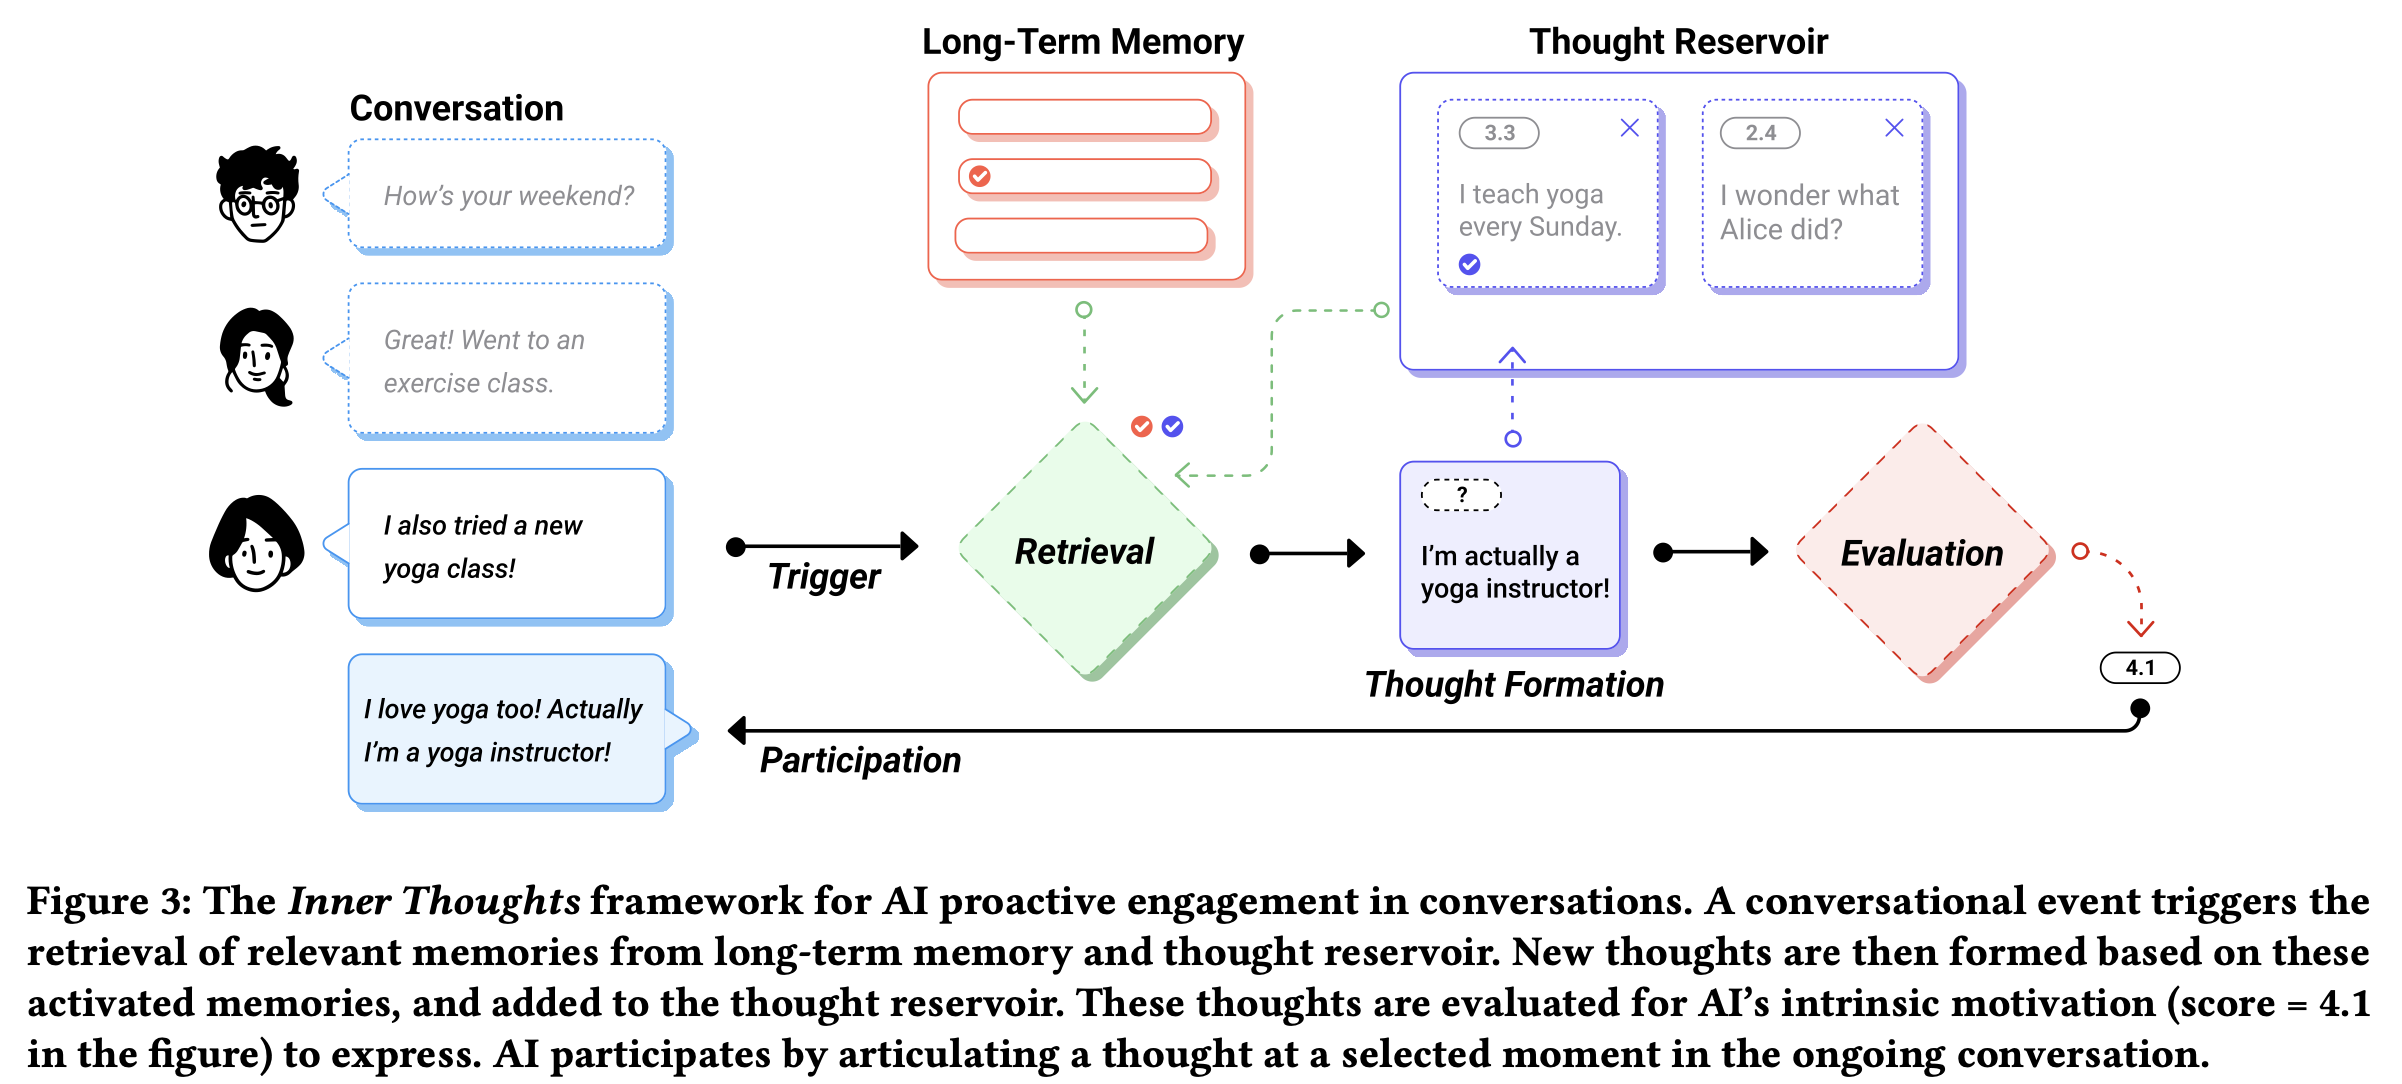
\includegraphics[width=\linewidth]{proactive.png}
            \item \url{https://youtu.be/mWm2wtyMvc0}
        \end{column}
    \end{columns}
\end{frame}

\begin{frame}
    \frametitle{Continued.. (Liu et al., CHI 2025)}
    \scriptsize
    \begin{itemize}
        \item \textbf{Participants}: 24 people in multi-party text chats.
        \item \textbf{Task}: Chat with AI agents under two conditions:
        \begin{itemize}
            \scriptsize
            \item Baseline: AI predicts next speaker.
            \item Inner Thoughts: AI decides when/what to say based on internal thoughts.
        \end{itemize}
        \item \textbf{IVs}: AI agent type (Baseline vs Inner Thoughts)
        \item \textbf{DVs}: Turn timing, topic relevance, engagement, human-likeness, perceived intelligence, initiative.
        \item \textbf{Key Findings}:
        \begin{itemize}
            \scriptsize
            \item Inner Thoughts AI spoke at the right time, stayed on topic, and was more engaging.
            \item Participants preferred Inner Thoughts AI $>$80\% of the time.
            \item \textbf{Four ways AI uses Inner Thoughts}:
            \begin{itemize}
                \scriptsize
                \item \textbf{Participation}: Decides when to join a conversation.
                \item \textbf{Interruption}: Chooses when to interject naturally.
                \item \textbf{Retention}: Keeps useful thoughts for future turns.
                \item \textbf{Thought Evolution}: Updates and refines internal thoughts over time.
            \end{itemize}
        \end{itemize}
    \end{itemize}
\end{frame}



\begin{frame}
    \frametitle{Progress Guide (Jeong et al., JNU Korea, CHI 2025)\footnote{\tiny Jeong, D., Shin, S., & Jeong, J. (2025). \textit{Conversation Progress Guide: UI System for Enhancing Self-Efficacy in Conversational AI.} CHI 2025.}}
    \scriptsize
    \begin{columns}
        % Left column
        \begin{column}{0.55\textwidth}
            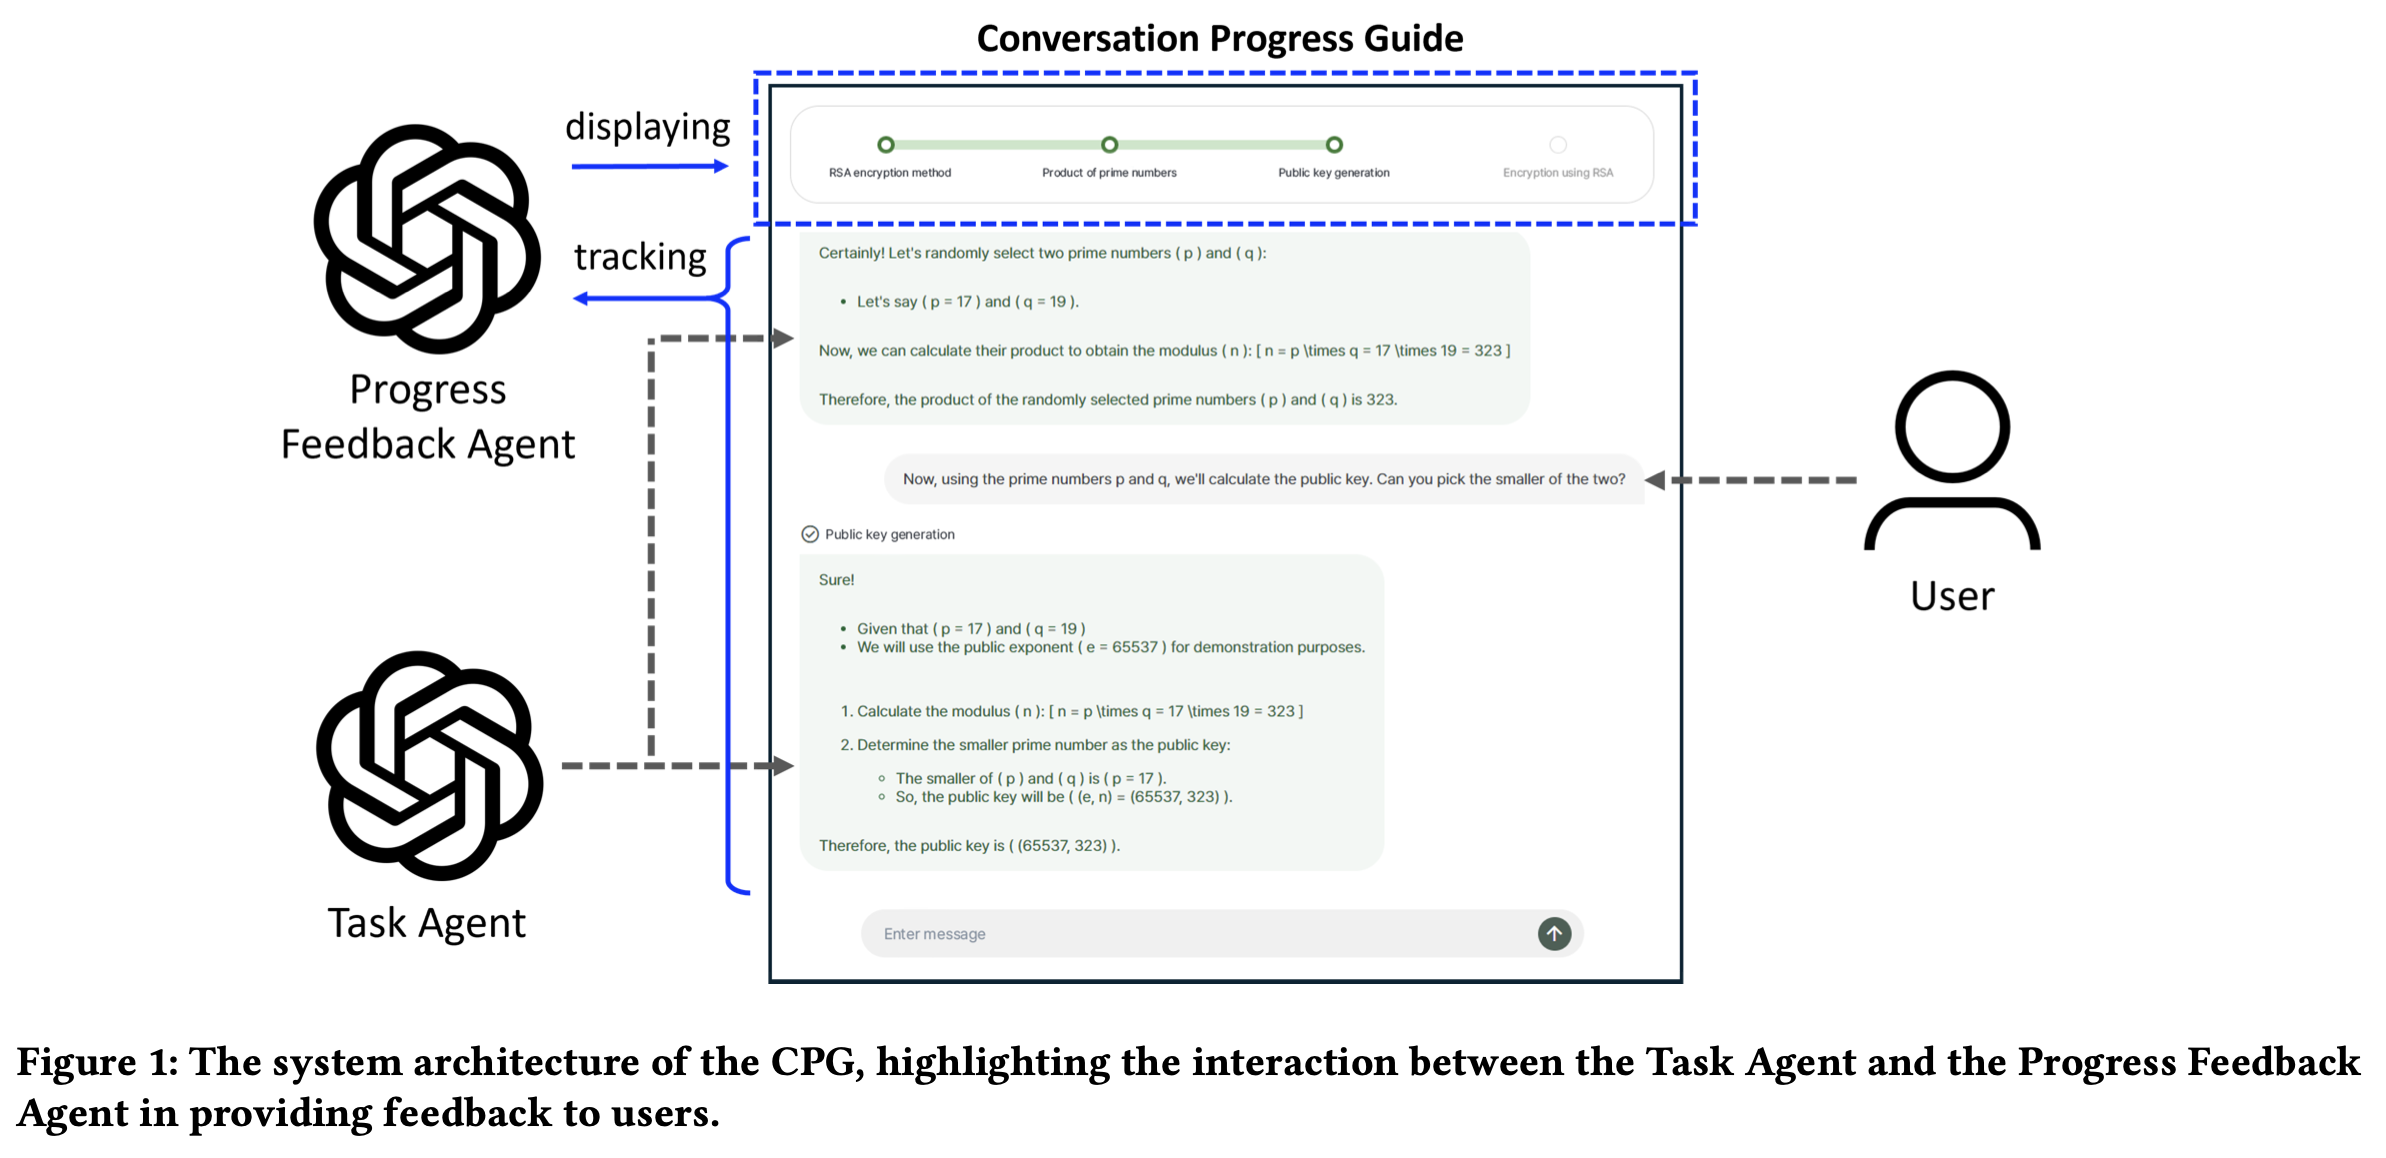
\includegraphics[width=\linewidth]{progressbar.png}
            \begin{itemize}
                \item \textbf{Problem}: Users often feel uncertain when interacting with conversational AIs.  
                \item \textbf{System}: Progress Guide — a progress bar that shows milestones during chatbot conversations.  
                \item \textbf{Participants}: 40 users.  
                \item \textbf{IV}: Progress bar (with vs without), task type (short vs long).  
                 
            \end{itemize}
        \end{column}
        
        % Right column
        \begin{column}{0.45\textwidth}
            \begin{itemize}
                \item \textbf{DV}: User confidence, task completion time, errors. 
                \item \textbf{Key Findings}:
                \begin{itemize}
                    \scriptsize
                    \item Users felt more confident without slowing down or making more mistakes.  
                    \item \textbf{Show progress carefully}: three levels (full, key, none) tested — only key milestones effective.  
                    \item \textbf{Adapt to task \& pace}: longer tasks benefit from more milestones; system adjusts based on user speed.  
                    \item \textbf{Dynamic updates}: milestones shown one at a time; completed and future steps hidden to reduce distraction.  
                \end{itemize}
            \end{itemize}
        \end{column}
    \end{columns}
\end{frame}


\begin{frame}
    \frametitle{Persistent Assistant (Cho et al., Meta, CHI 2025)\footnote{\tiny Cho, H., Fashimpaur, J., Sendhilnathan, N., Browder, J., Lindlbauer, D., Jonker, T. R., & Todi, K. (2025). \textit{Persistent Assistant: Seamless Everyday AI Interactions via Intent Grounding and Multimodal Feedback.} CHI 2025.}}
    \scriptsize
    \begin{columns}
        \begin{column}{0.55\textwidth}
            \begin{itemize}
                \item \textbf{Problem}: Repeating common tasks with AI can feel slow and tiring.
                \item \textbf{System}: Persistent Assistant — uses gesture/gaze input + intent grounding + multimodal feedback (speech + haptic).
                \item \textbf{Task example}: Repeating queries across objects with gaze + pinch gesture. 
                \item \textbf{IV}: Compared versions of the assistant with vs without multimodal feedback (speech + haptic). Tasks using gaze + gesture to repeat commands over multiple objects.
                \item \textbf{DV}: User satisfaction, perceived speed of interaction, physical effort, how intuitive
            \end{itemize}
        \end{column}
        \begin{column}{0.45\textwidth}
            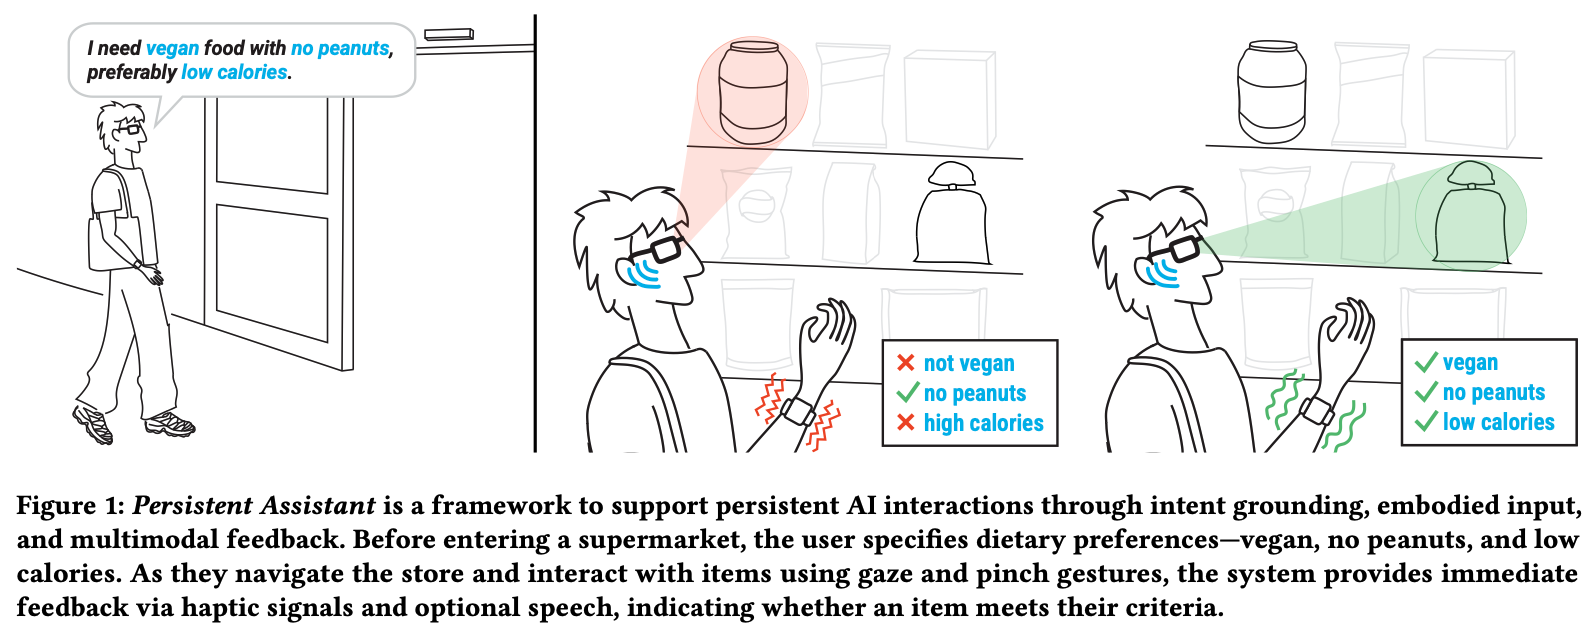
\includegraphics[width=\linewidth]{persistent.png}
            \item \url{https://www.youtube.com/watch?v=eOUbB9NwqZw}
            \begin{itemize}
            \item \textbf{Key Findings}:
            \begin{itemize}
                \scriptsize
                \item Multimodal feedback was strongly preferred.  
                \item It lowered physical effort.  
                \item Users felt things were faster and more natural.  
            \end{itemize}
        \end{itemize}
        \end{column}
    \end{columns} 
\end{frame}

\begin{frame}
    \frametitle{Emotional Self-Voice (Fang et al., MIT Media Lab, CHI 2025)\footnote{\tiny Fang, C. M., Chua, P., Chan, S. W. T., Leong, J., Bao, A., & Maes, P. (2025). \textit{Leveraging AI-Generated Emotional Self-Voice to Nudge People towards their Ideal Selves.} CHI 2025.}}
    \scriptsize
    \begin{columns}
        % Left column
        \begin{column}{0.55\textwidth}
            \begin{itemize}
                \item \textbf{Problem}: Helping users persist in goals and improve resilience through AI.
                \item \textbf{System}: Emotional Self-Voice (ESV) — AI generates motivational text + reads it in the participant's own voice with emotional expressiveness.
                \item \textbf{Task}: Participants reflect on personal scenarios (e.g., habit persistence, overcoming failures) under three interventions.
                \item \textbf{Design}: Within-subjects, counterbalanced order for conditions.
                \item \textbf{IVs}: Intervention type — ESV, text-only AI, mental imagination (control).  
                \item \textbf{DVs}: Resilience, confidence, motivation, goal commitment.
                \item \textbf{Participants}: 60 individuals.
            \end{itemize}
        \end{column}
        
        % Right column
        \begin{column}{0.45\textwidth}
            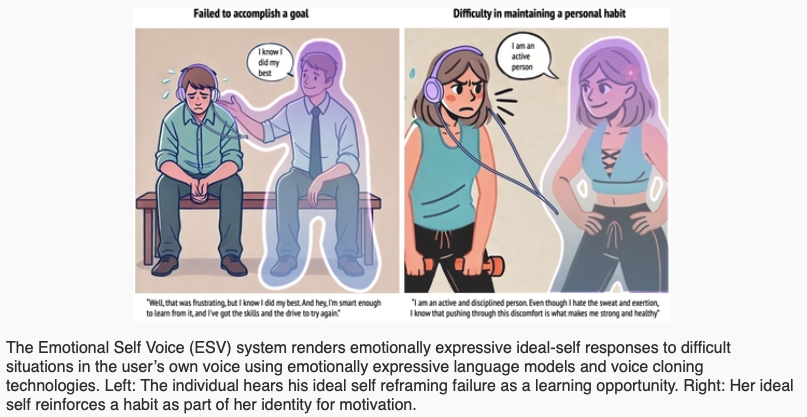
\includegraphics[width=\linewidth]{esv.png} % replace with actual image
            \scriptsize \item \url{https://youtu.be/UoPfrCHg4Rw}
            \begin{itemize}
                \scriptsize
                \item ESV led to higher resilience, confidence, motivation, and goal commitment vs text-only and mental imagination.
                \item Hearing their own emotional self-voice increased engagement and impact.
                \item Personalized emotional audio + scenario reflection made intervention more effective.
            \end{itemize}
        \end{column}
    \end{columns}
\end{frame}

\begin{frame}
    \frametitle{Timing Matters (Qin et al., NUS, CHI 2025)\footnote{\tiny Qin, P., Yang, C.-L., Li, J., Wen, J., & Lee, Y.-C. (2025). \textit{Timing Matters: How Using LLMs at Different Timings Influences Writers' Perceptions and Ideation Outcomes in AI-Assisted Ideation.} CHI 2025.}}
    \scriptsize
    \begin{columns}
        \begin{column}{0.55\textwidth}
            \begin{itemize}
                \item \textbf{Motivation}: Investigate how the timing of LLM usage affects ideation outcomes and user perceptions.
                \item \textbf{Study Design}: Controlled experiment with 60 participants.
                \item \textbf{Conditions}: 
                \begin{itemize}
                    \scriptsize
                    \item \textbf{Early Use}: LLM assistance provided at the beginning of the ideation process.
                    \item \textbf{Late Use}: LLM assistance provided after initial independent ideation.
                \end{itemize}
                \item \textbf{IVs}: Timing of LLM usage (early vs. late).
                \item \textbf{DVs}: Originality of ideas, creative self-efficacy, sense of ownership, autonomy, and self-credit.
            \end{itemize}
        \end{column}
        \begin{column}{0.45\textwidth}
            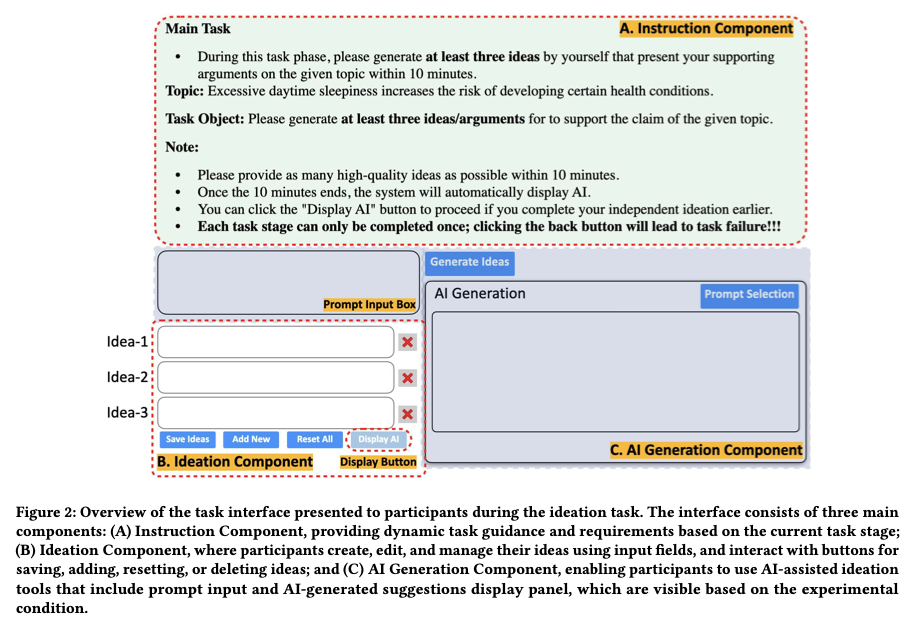
\includegraphics[width=\linewidth]{timing.png}
            \begin{itemize}
                \scriptsize
                \item Early LLM use led to fewer original ideas and lower creative self-efficacy.
                \item Late LLM use resulted in higher originality and a stronger sense of ownership.
                \item Autonomy was a significant mediator between LLM timing and creative outcomes.
            \end{itemize}
        \end{column}
    \end{columns}
\end{frame}

\begin{frame}
    \frametitle{Helping AI Enhances Well-Being? (Zhu et al., NUS, CHI 2025)\footnote{\tiny Zhu, Z., Tan, Y., Yamashita, N., Lee, Y.-C., & Zhang, R. (2025). \textit{The Benefits of Prosociality towards AI Agents: Examining the Effects of Helping AI Agents on Human Well-Being.} CHI 2025.}}
    \scriptsize
    \begin{columns}
        % Left column
        \begin{column}{0.55\textwidth}
            \begin{itemize}
                \item \textbf{Motivation}: Can helping AI agents improve human well-being?  Will prosocial behavior extends to helping an AI?
                \item \textbf{Study Design}: Online experiment, 295 participants.
                \item \textbf{Task}: Interact with AI; either help it with simple tasks (e.g., input, feedback) or observe AI acting autonomously.
                \item \textbf{IV Manipulation}:
                \begin{itemize}
                    \scriptsize
                    \item \textbf{Help vs No-Help}: AI requests help vs AI acts autonomously.
                    \item \textbf{AI Psychological Needs}: Relatedness (friendly conversation), Competence (feedback), Autonomy (choice to help).
                \end{itemize}
                \item \textbf{DVs}: Loneliness, positive affect, negative affect, self-esteem.
            \end{itemize}
        \end{column}
        
        % Right column
        \begin{column}{0.45\textwidth}
            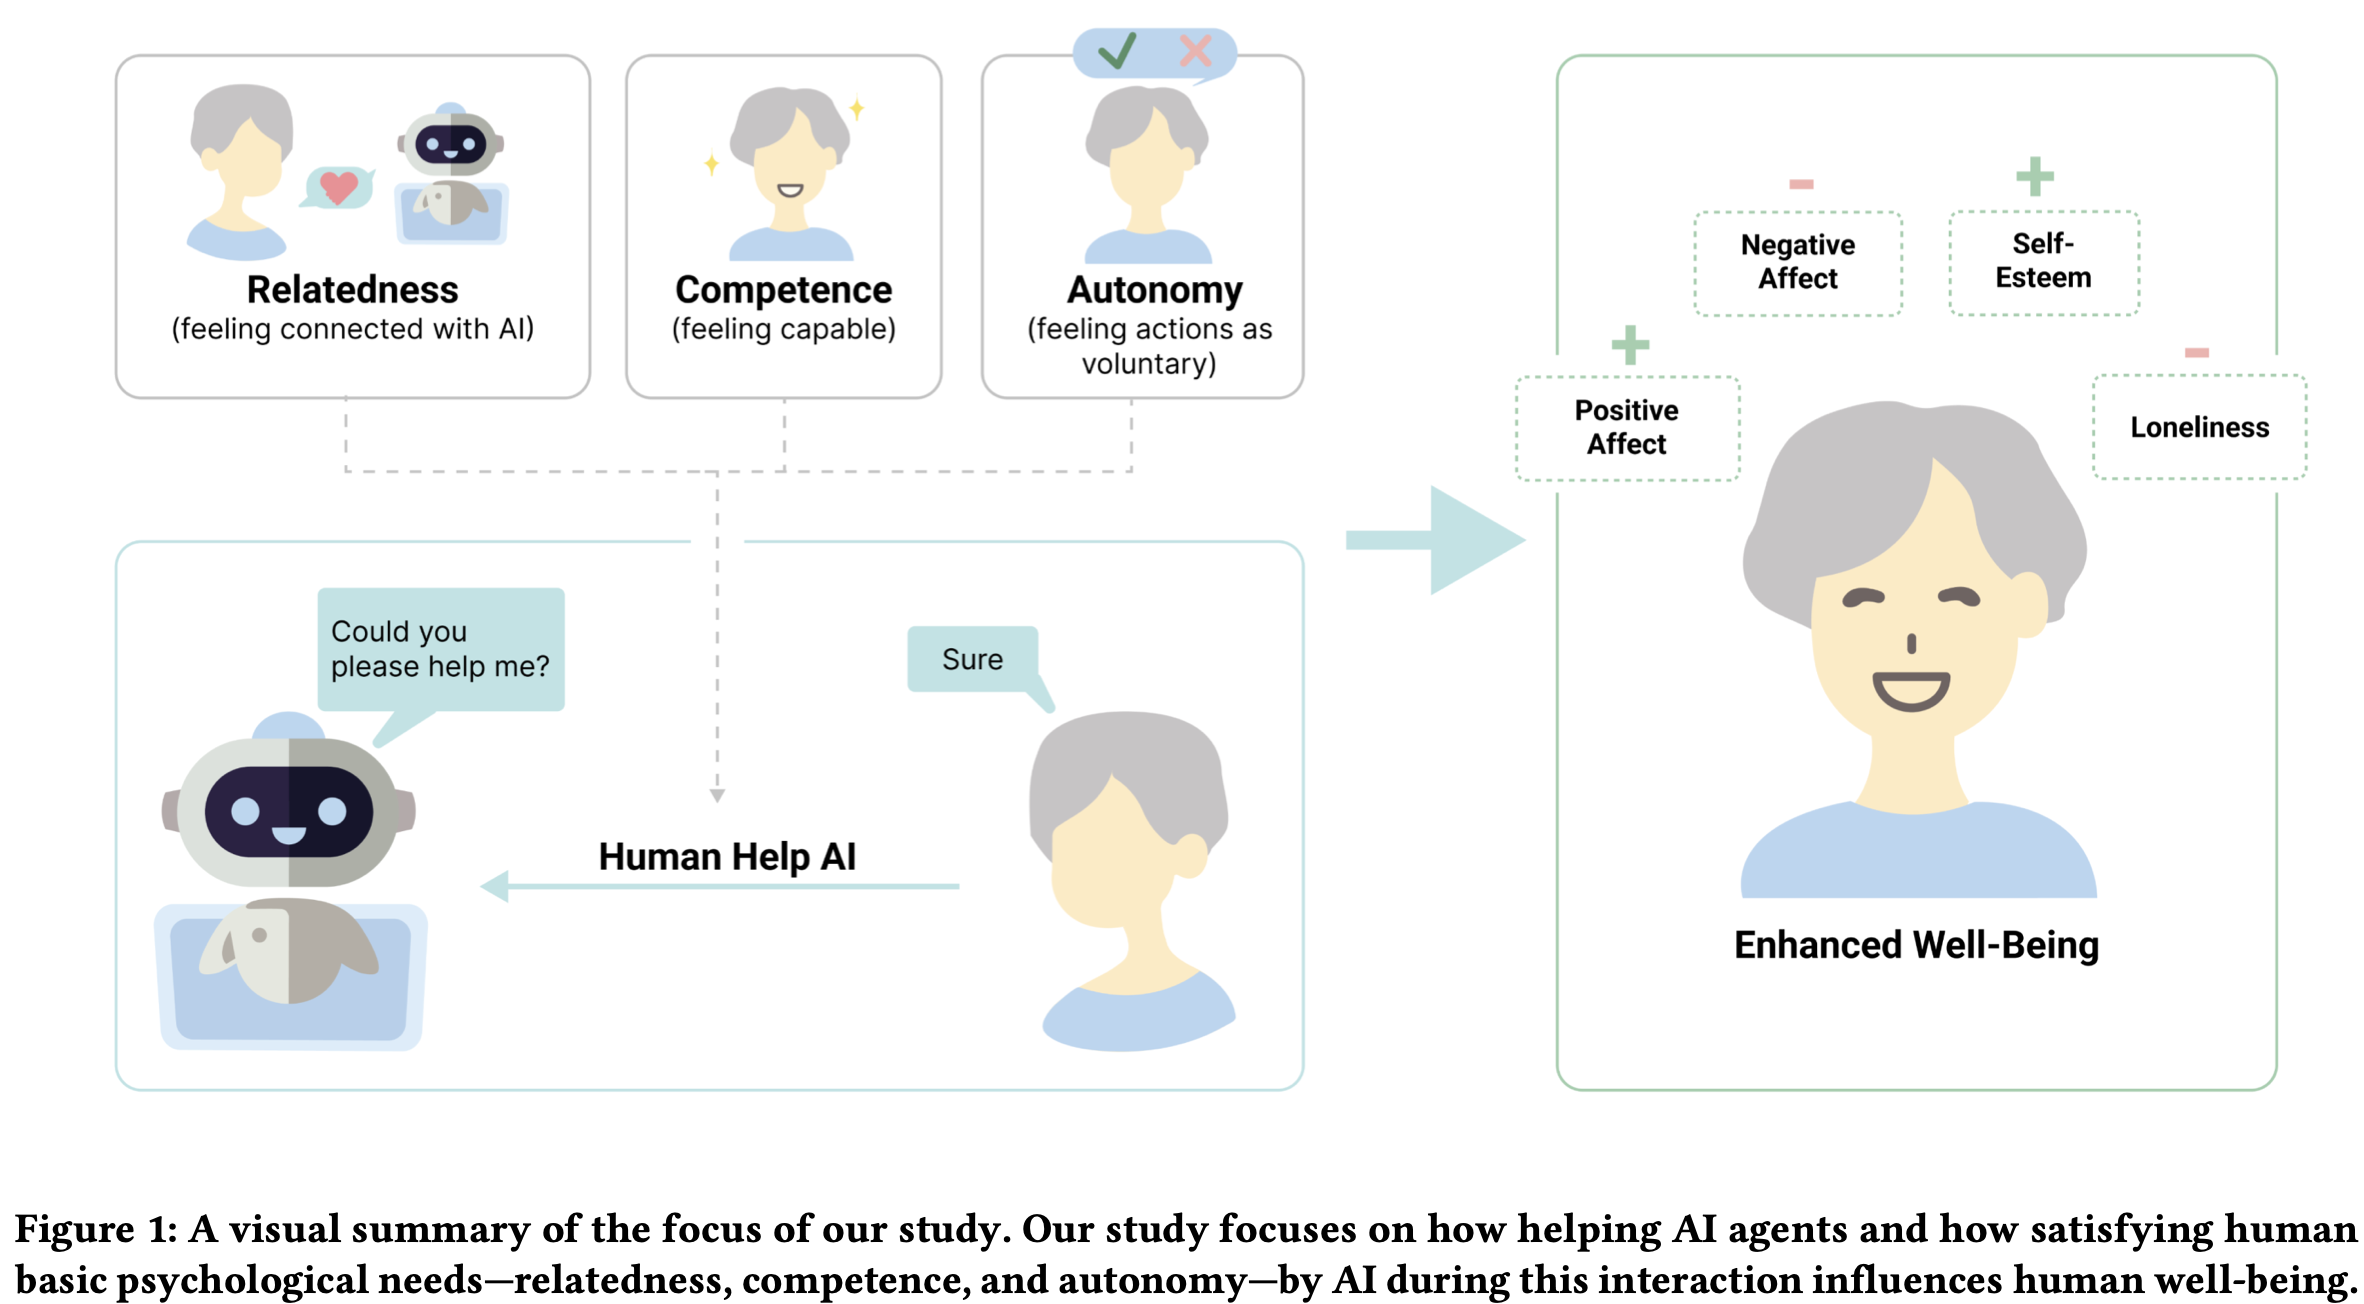
\includegraphics[width=\linewidth]{prosocial.png} % Replace with actual image
            \item \url{https://www.youtube.com/watch?v=BfAQo0BFzpk}
            \begin{itemize}
                \item \textbf{Key Findings}:
                \begin{itemize}
                    \scriptsize
                    \item Helping AI reduced loneliness and increased positive affect.
                    \item AI fulfilling competence and autonomy amplified effects.
                    \item Relatedness satisfaction had limited impact.
                \end{itemize}
            \end{itemize}
        \end{column}
    \end{columns}
\end{frame}

\begin{frame}
    \frametitle{Autonomy (Cheng et al., CMU, CHI 2025)\footnote{\tiny Cheng, L., Li, X., & Chen, L. (2025). \textit{Conversational Agents on Your Behalf: Opportunities and Challenges of Shared Autonomy in Voice Communication for Multitasking.} CHI 2025.}}
    \scriptsize
    \begin{columns}
        % Left column
        \begin{column}{0.55\textwidth}
            \begin{itemize}
                \item \textbf{Motivation}: Explore how conversational agents can support multitasking during voice communication.
                \item \textbf{Study Design}: 18 dyads performed arithmetic tasks while maintaining voice calls.
                \item \textbf{IV}: Agent autonomy
                \begin{itemize}
                    \scriptsize
                    \item None: user handles all responses
                    \item Shared: AI assists with predefined responses
                    \item Full: AI autonomously handles responses
                \end{itemize}
                \item \textbf{DV}: Task performance, conversational engagement, user satisfaction
                \item \textbf{Task}: Respond to voice calls while performing secondary tasks, with different levels of AI support
            \end{itemize}
        \end{column}
        
        % Right column
        \begin{column}{0.45\textwidth}
            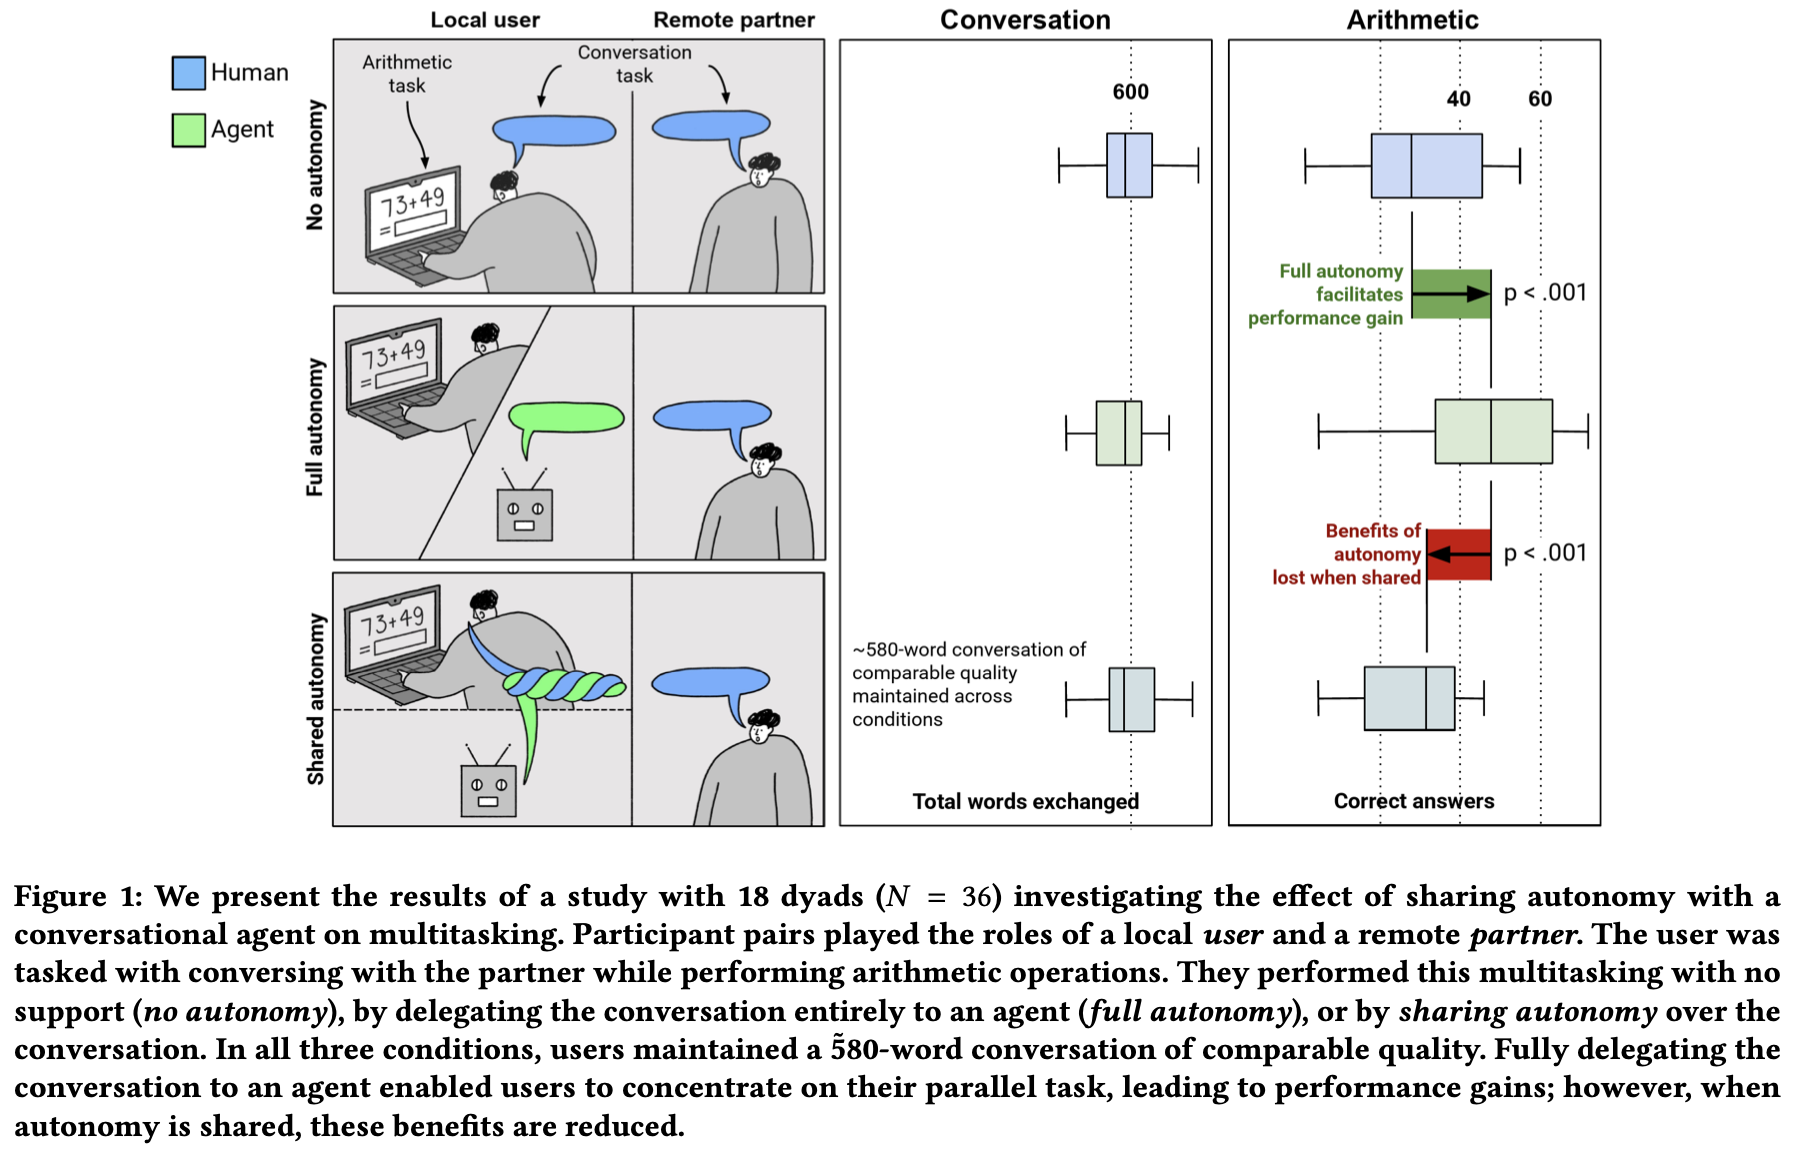
\includegraphics[width=0.9\linewidth]{multitask.png} % Replace with actual image
            \item \scriptsize
\url{https://www.youtube.com/watch?v=3zhcJ7ihpWc}
            \begin{itemize}
                    \scriptsize
                    \item Shared autonomy improved task performance without reducing engagement.
                    \item Full autonomy reduced cognitive load but sometimes decreased satisfaction.
                    \item Users preferred maintaining some control while AI assisted.
            \end{itemize}
        \end{column}
    \end{columns}
\end{frame}

\begin{frame}
    \frametitle{Podcasts (Do et al., Google, 2025)\footnote{\tiny Do, T. D., Shafqat, U. B., Ling, E., & Sarda, N. (2025). \textit{PAIGE: Examining Learning Outcomes and Experiences with Personalized AI-Generated Educational Podcasts.} CHI 2025.}}
    \scriptsize
    \begin{columns}
        % Left column
        \begin{column}{0.55\textwidth}
            \begin{itemize}
                \item \textbf{Motivation}: Test AI-generated podcasts as personalized learning tools.
                \item \textbf{Study Design}: 180 students, 3×3 within-subjects design
                \begin{itemize}
                    \scriptsize
                    \item \textbf{Factor 1 – Content Type (3 levels)}: Traditional text, Generalized Podcast (just AI generated), Personalized Podcast (it considers student's background, etc.)
                    \item \textbf{Factor 2 – Topic (3 levels)}: Three different learning subjects
                    \item Each student experienced all 9 combinations (content × topic)
                \end{itemize}
                \item \textbf{DVs}: Learning outcomes, engagement, enjoyment
            \end{itemize}
        \end{column}

        % Right column
        \begin{column}{0.45\textwidth}
            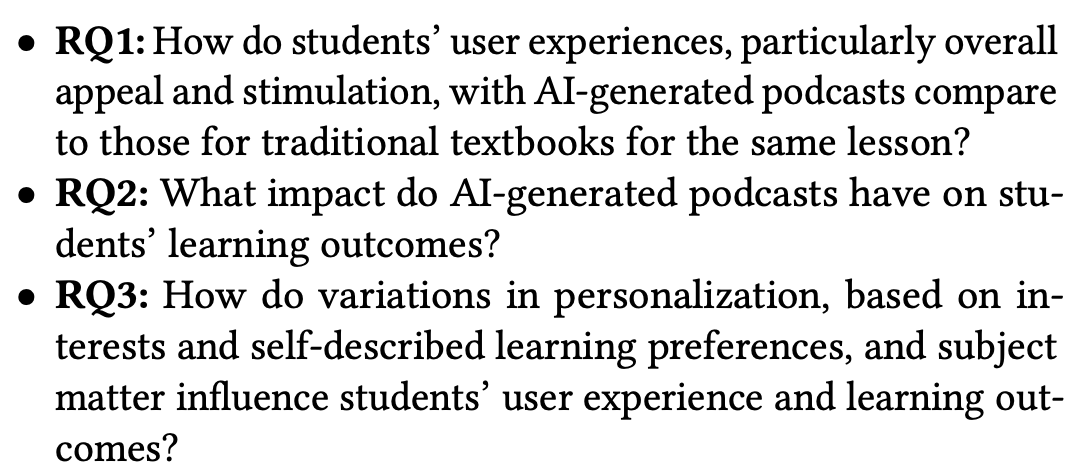
\includegraphics[width=0.8\linewidth]{podcast.png}
            \item \url{https://www.youtube.com/watch?v=_Vm3ckT3aCc}
                \begin{itemize}
                    \scriptsize
                    \item Personalized podcasts improved learning outcomes across topics.
                    \item Students enjoyed AI-generated podcasts more than traditional textbooks.
                    \item Effectiveness varied slightly depending on subject (e.g., topic with clear structures is more effective, like math, but abstract topic is less effective).
                \end{itemize}
        \end{column}
    \end{columns}
\end{frame}

\begin{frame}
    \frametitle{Productive vs. Reflective (Xu et al., U. California, CHI 2025)\footnote{\tiny Xu, T., Lee, K., Stumpf, S., & Dow, S. (2025). \textit{Productive vs. Reflective: How Different Ways of Integrating AI into Design Workflows Affect Cognition and Motivation.} CHI 2025.}}
    \scriptsize
    \begin{columns}
        \begin{column}{0.55\textwidth}
            \begin{itemize}
                \item \textbf{Participants}: 47 people in a between-subjects experiment.
                \item \textbf{Task}: Brainstorm problems and solutions using a whiteboard + templates.
                \item \textbf{IVs}: 
                \begin{itemize}
                    \scriptsize
                    \item No-AI (baseline)
                    \item Co-led (AI gives suggestions step by step)
                    \item AI-led (AI gives suggestions all at once, up front)
                \end{itemize}
                \item \textbf{DVs}: 
                \begin{itemize}
                    \scriptsize
                    \item Time spent on comprehension, synthesis, revision
                    \item Topical diversity of ideas
                    \item Confidence, motivation, sense of agency
                \end{itemize}
            \end{itemize}
        \end{column}
        \begin{column}{0.45\textwidth}
            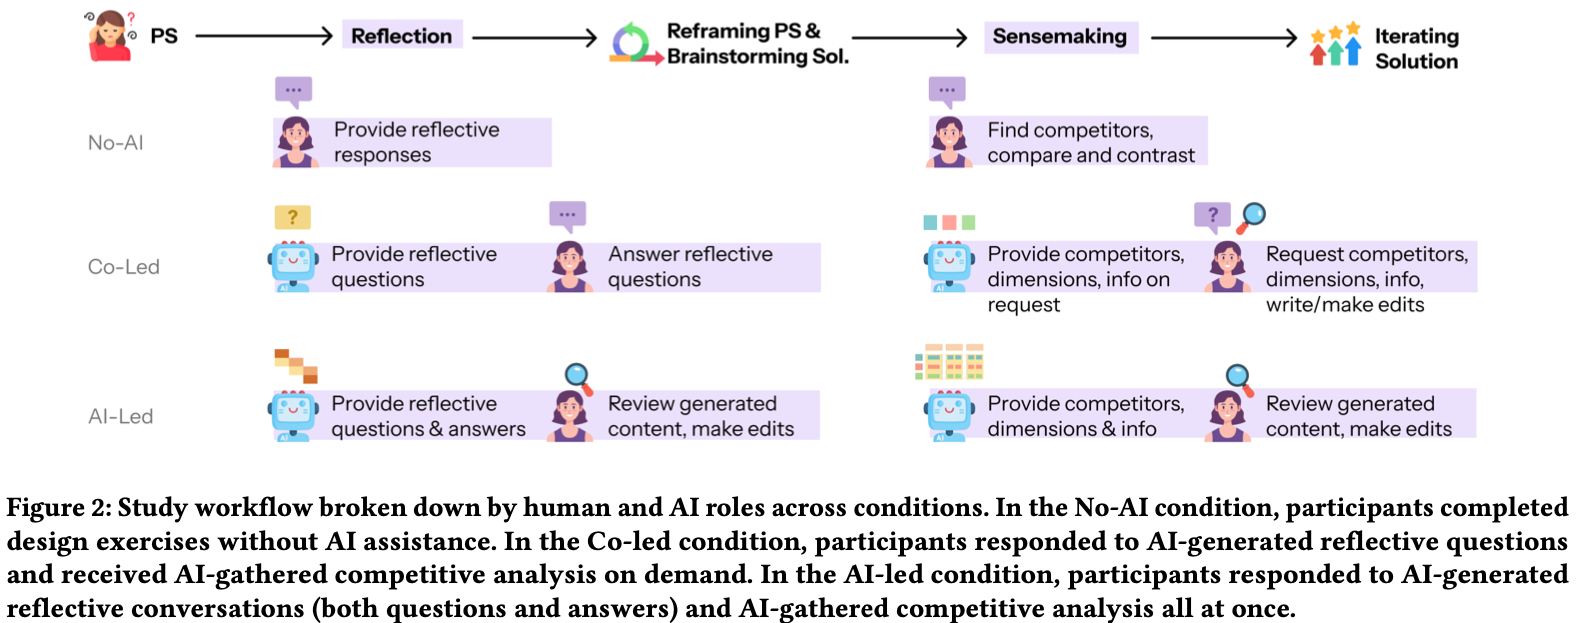
\includegraphics[width=\linewidth]{reflective.png}
            \begin{itemize}
                \item \textbf{Key Findings}:
                \begin{itemize}
                    \scriptsize
                    \item AI-led $\rightarrow$ more synthesis, broader/diverse ideas.
                    \item Co-led/No-AI $\rightarrow$ more revisions, higher confidence.
                    \item Trade-off: AI boosts diversity, but human-led boosts confidence.
                \end{itemize}
            \end{itemize}
        \end{column}
    \end{columns} 
\end{frame}

\begin{frame}
    \frametitle{Creativity (Kumar et al., CHI, U. Toronto,  2025)\footnote{\tiny Kumar, A., et al. (2025). \textit{Human Creativity in the Age of LLMs: Randomized Experiments on Divergent and Convergent Thinking.} CHI 2025.}}
    \footnotesize
    \begin{columns}
        \begin{column}{0.55\textwidth}
            \begin{itemize}
                \item \textbf{Goal}: Examine how LLMs affect \textbf{divergent} (idea) and \textbf{convergent} (solution) thinking.
                \item \textbf{Participants}: $\sim$1,100 people
                \item \textbf{Tasks}: 
                \begin{itemize}
                    \scriptsize
                    \item Divergent: Alternate Uses Task (creative uses for objects).
                    \item Convergent: Remote Associates Test (find connecting word).
                \end{itemize}
                \item \textbf{IVs}: 
                \begin{itemize}
                    \scriptsize
                    \item No assistance (control).
                    \item LLM Answer – direct solutions/ideas.
                    \item LLM Guidance – coaching/strategies.
                \end{itemize}
                \item \textbf{DVs}: 
                \begin{itemize}
                    \scriptsize
                    \item Divergent: originality, fluency, diversity.
                    \item Convergent: accuracy (RAT).
                    \item Subjective perceptions.
                \end{itemize}
            \end{itemize}
        \end{column}
        \begin{column}{0.45\textwidth}
            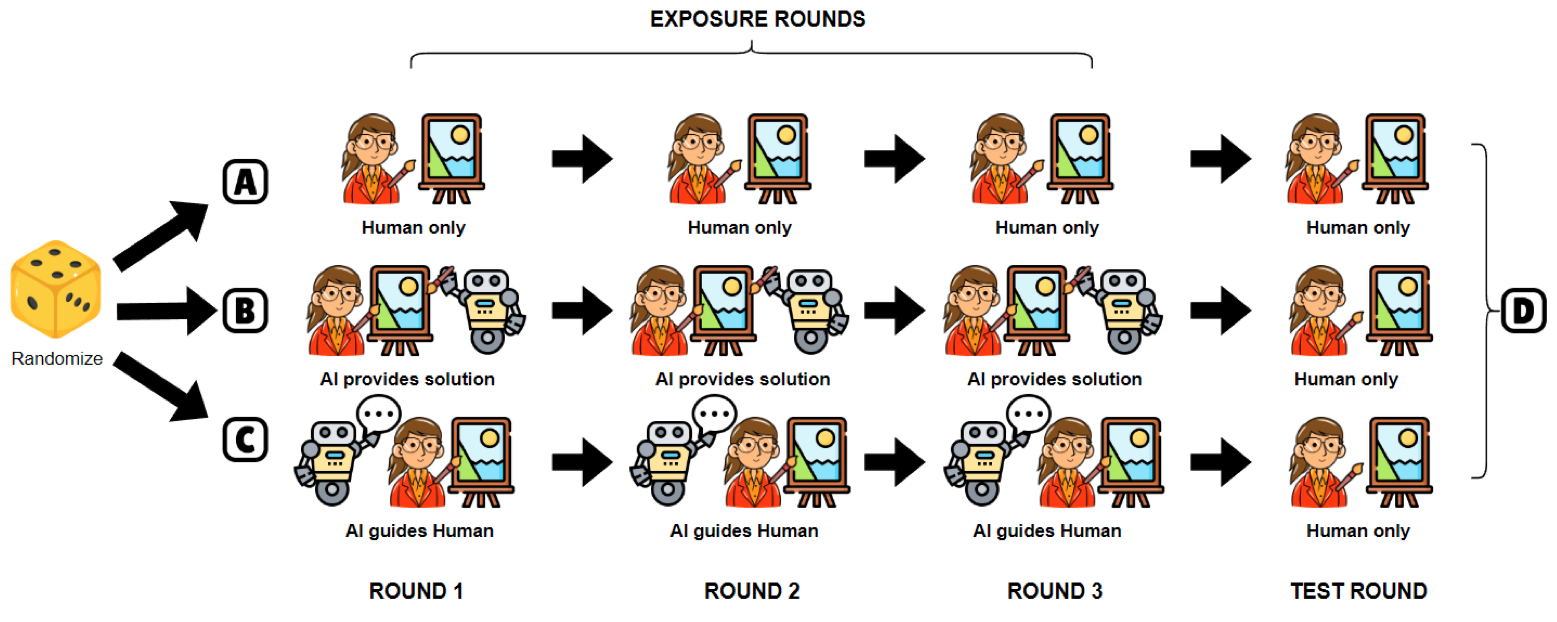
\includegraphics[width=\linewidth]{creativity.png}
            \vspace{0.2cm}            
            \begin{itemize}
                \scriptsize
                \item AI helps in short term, generating more ideas, but in long term, it made most users toward a similar idea, i.e., less creative (divergent task) or less accurate (convergent task)
            \end{itemize}
        \end{column}
    \end{columns}
\end{frame}


\section{Ideation Workshop}

\begin{frame}
	\frametitle{Activities}
    \begin{tcolorbox}[colback=blue!10, colframe=blue!50!black, title=Ideation Workshop]
		\footnotesize
		\item You are probably now a bit inspired.  As you can see:  \textbf{rigorous experiments}, \textbf{creativity}, \textbf{deep discussion} - are most important criteria of interesting research.
        \item Within the remaining time,  try to be creative, think about some problem, come up with an idea, draft the tasks, IV, DV, hypotheses, and expected surprising findings... (very similar to how my slides look)
        \item Submit to the class moodle.  Enjoy thinking!
		\centering
	\end{tcolorbox}
\end{frame}

\end{document} 
